\documentclass[a4paper]{article}

\usepackage[english]{babel}
\usepackage[T1]{fontenc}
\usepackage{amsmath}
\usepackage{graphicx}
\usepackage[colorinlistoftodos]{todonotes}
\usepackage{makeidx}
\usepackage{fullpage,xspace,setspace,lscape}
\makeindex

\renewcommand{\thefigure}{S\arabic{figure}}


\title{\huge\bfseries \vspace{2cm} The \textit{E. coli} molecular phenotype under different growth conditions \\ \vspace{0.7cm}
	\Large\bfseries Supplementary material \vspace{1.3cm}}


\author{
	\large\bfseries Mehmet U. Caglar, John R. Houser, Craig S. Barnhart, \\
	\large\bfseries Daniel R. Boutz, Sean M. Carroll, Aurko Dasgupta, Walter F. Lenoir,\\ 
	\large\bfseries Bartram L. Smith, Viswanadham Sridhara, Dariya K. Sydykova, \\
	\large\bfseries Drew Vander Wood, Christopher J. Marx, \\
	\large\bfseries Edward M. Marcotte*, Jeffrey E. Barrick*, Claus O. Wilke*}




\begin{document}
\maketitle
\newpage
	
	
	
\tableofcontents
\listoffigures
\listoftables

\newpage


\section*{Supplementary Figures associated with differentially expressed KEGG pathways}
\begin{figure}[!htb]
	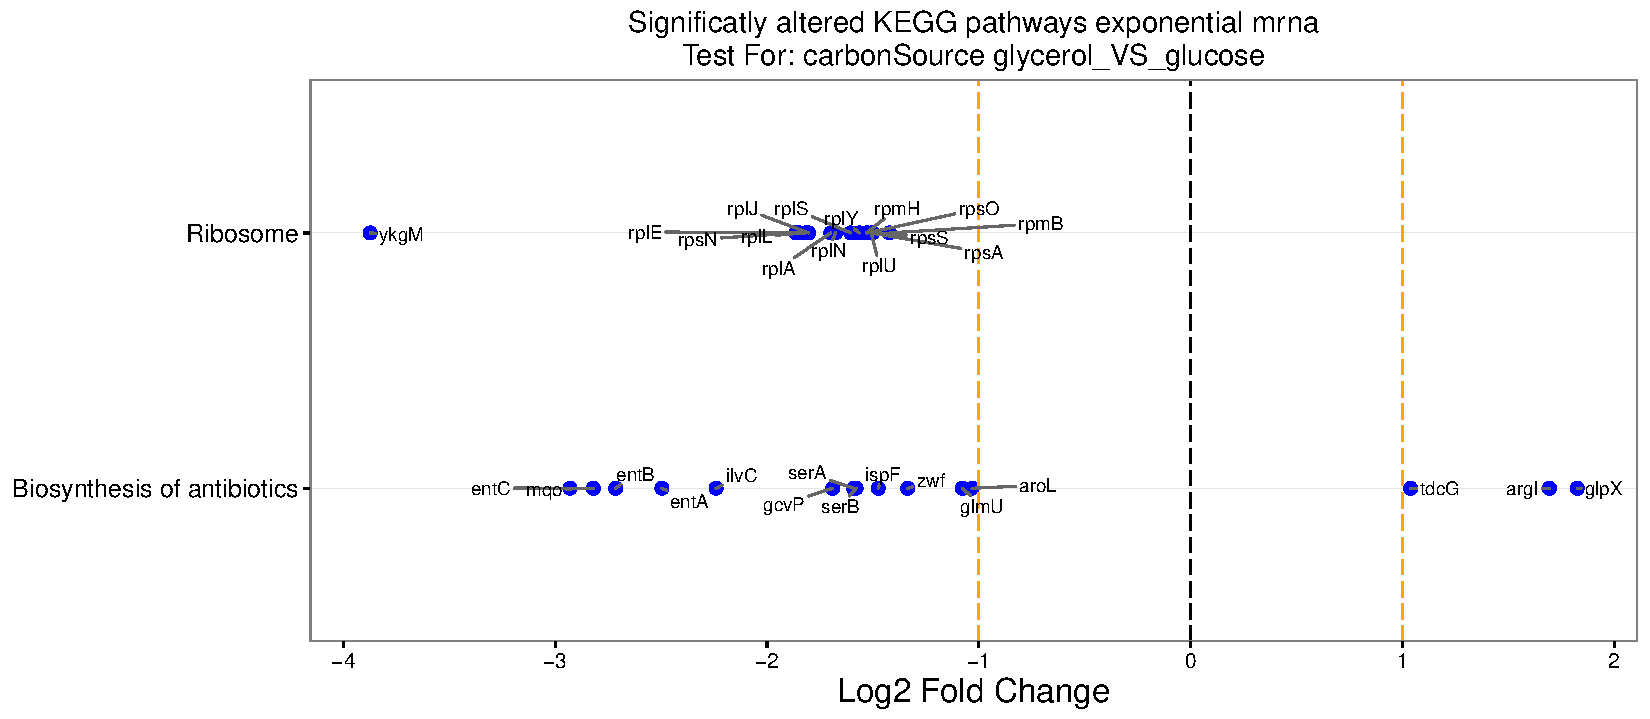
\includegraphics[width=1.0\textwidth]{../../d_figures/kegg_01.pdf}
	\caption[Significantly altered KEGG pathways for mRNA samples in exponential phase tested for glycerol against glucose]
	{\textbf{Significantly differentially expressed KEGG pathways and associated genes with glycerol as carbon source in exponential phase, as determined by mRNA abundances.} The top differentially expressed KEGG pathways are shown along the y axis, and the relative fold change of the corresponding genes is shown along the x axis. In figure we show up to 10 most significantly changed pathways and for each pathway we show up to 15 of the most significantly changing genes.}
\end{figure}

\clearpage
\begin{figure}
	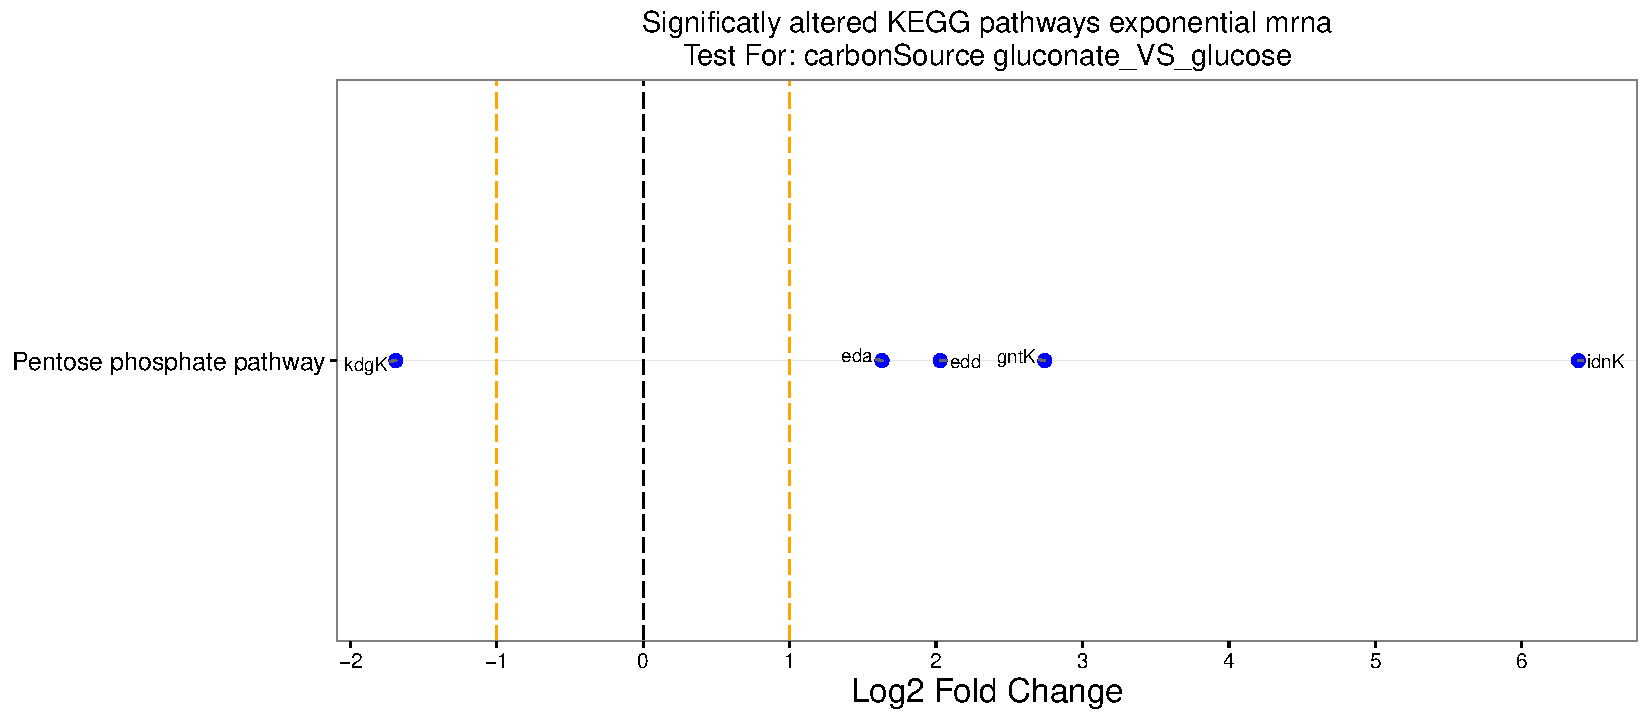
\includegraphics[width=1.0\textwidth]{../../d_figures/kegg_02.pdf}
	\caption[Significantly altered KEGG pathways for mRNA samples in exponential phase tested for  against glucose]
	{\textbf{Significantly differentially expressed KEGG pathways and associated genes with gluconate as carbon source in exponential phase, as determined by mRNA abundances.} The top differentially expressed KEGG pathways are shown along the y axis, and the relative fold change of the corresponding genes is shown along the x axis. In figure we show up to 10 most significantly changed pathways and for each pathway we show up to 15 of the most significantly changing genes.}
\end{figure}

\clearpage
\begin{figure}
	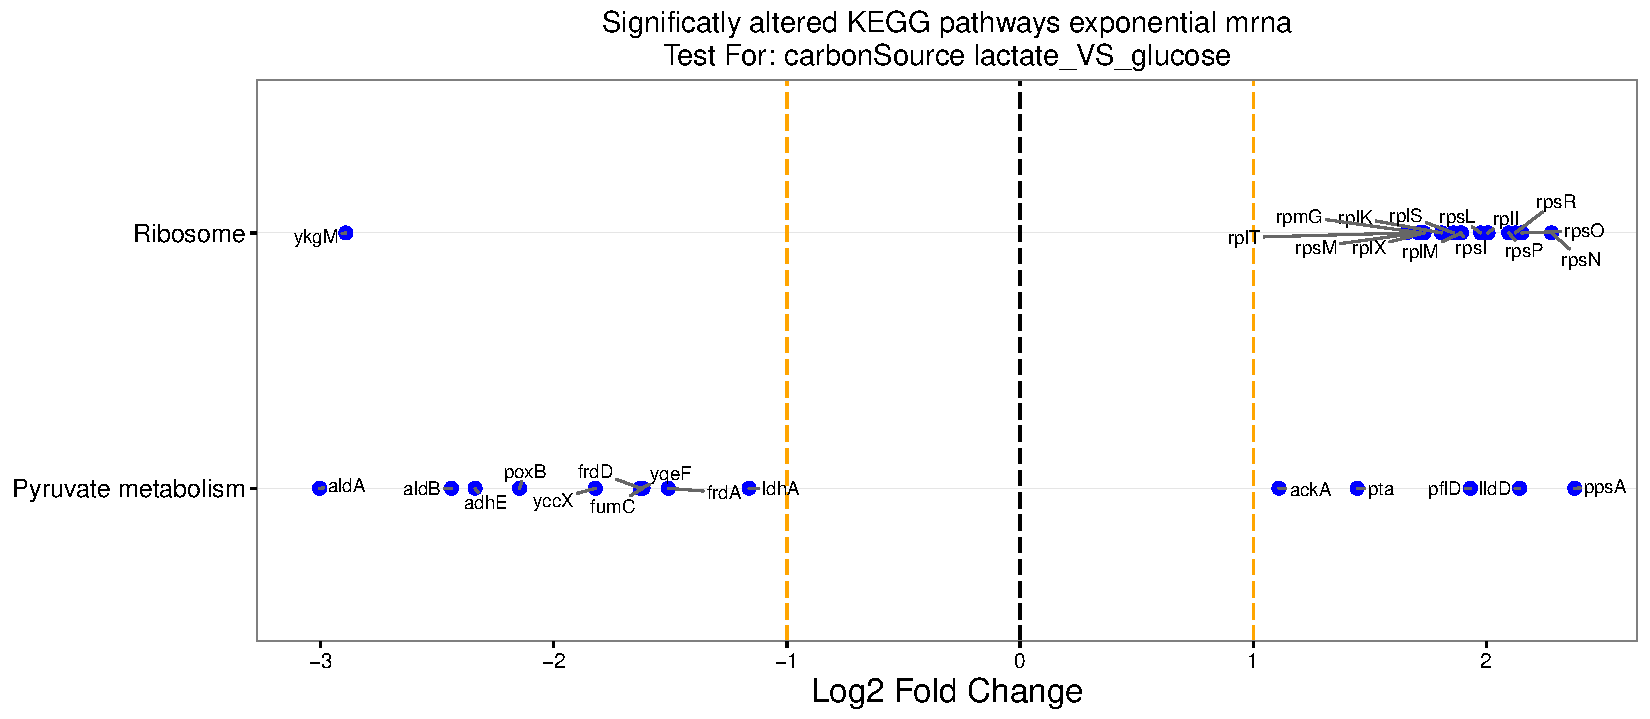
\includegraphics[width=1.0\textwidth]{../../d_figures/kegg_03.pdf}
	\caption[Significantly altered KEGG pathways for mRNA samples in exponential phase tested for lactate against glucose]
	{\textbf{Significantly differentially expressed KEGG pathways and associated genes with lactate as carbon source in exponential phase, as determined by mRNA abundances.} The top differentially expressed KEGG pathways are shown along the y axis, and the relative fold change of the corresponding genes is shown along the x axis. In figure we show up to 10 most significantly changed pathways and for each pathway we show up to 15 of the most significantly changing genes.}
\end{figure}

\clearpage
\begin{figure}
	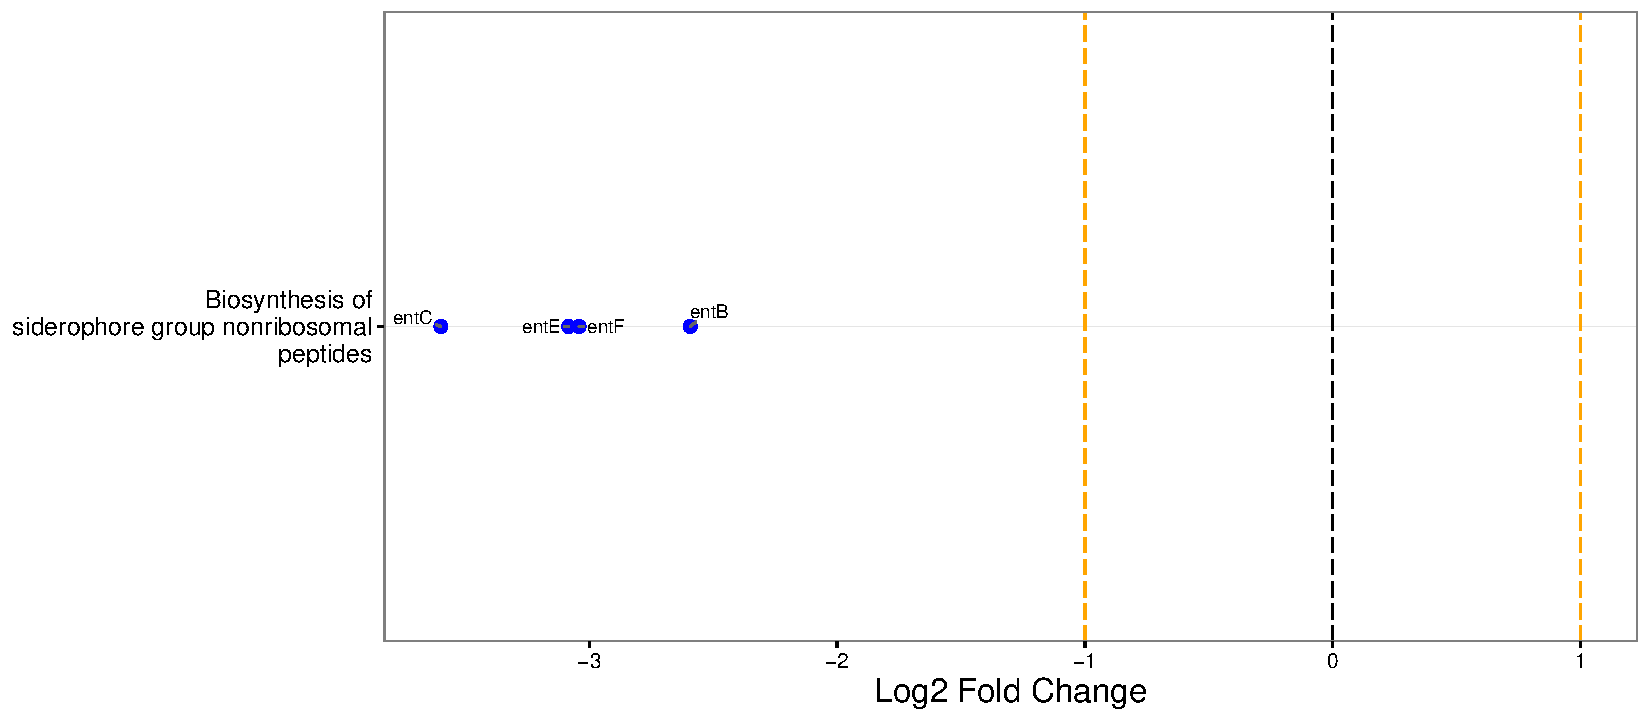
\includegraphics[width=1.0\textwidth]{../../d_figures/kegg_04.pdf}
	\caption[Significantly altered KEGG pathways for protein samples in exponential phase tested for gluconate against glucose]
	{\textbf{Significantly differentially expressed KEGG pathways and associated genes with gluconate as carbon source in exponential phase, as determined by protein abundances.} The top differentially expressed KEGG pathways are shown along the y axis, and the relative fold change of the corresponding genes is shown along the x axis. In figure we show up to 10 most significantly changed pathways and for each pathway we show up to 15 of the most significantly changing genes.}
\end{figure}

\clearpage
\begin{figure}
	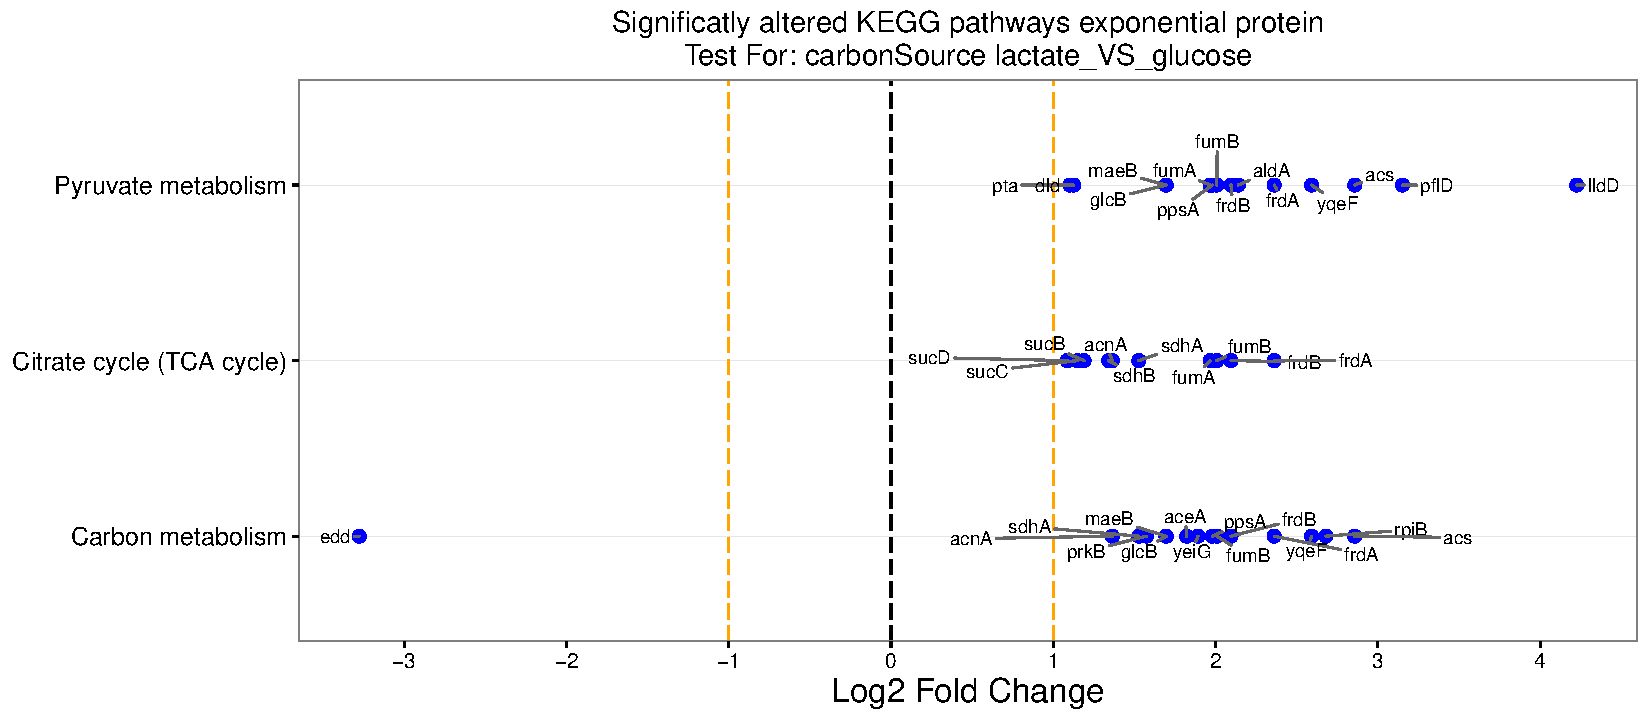
\includegraphics[width=1.0\textwidth]{../../d_figures/kegg_05.pdf}
	\caption[Significantly altered KEGG pathways for protein samples in exponential phase tested for lactate against glucose]
	{\textbf{Significantly differentially expressed KEGG pathways and associated genes with lactate as carbon source in exponential phase, as determined by protein abundances.} The top differentially expressed KEGG pathways are shown along the y axis, and the relative fold change of the corresponding genes is shown along the x axis. In figure we show up to 10 most significantly changed pathways and for each pathway we show up to 15 of the most significantly changing genes.}
\end{figure}

\clearpage
\begin{figure}
	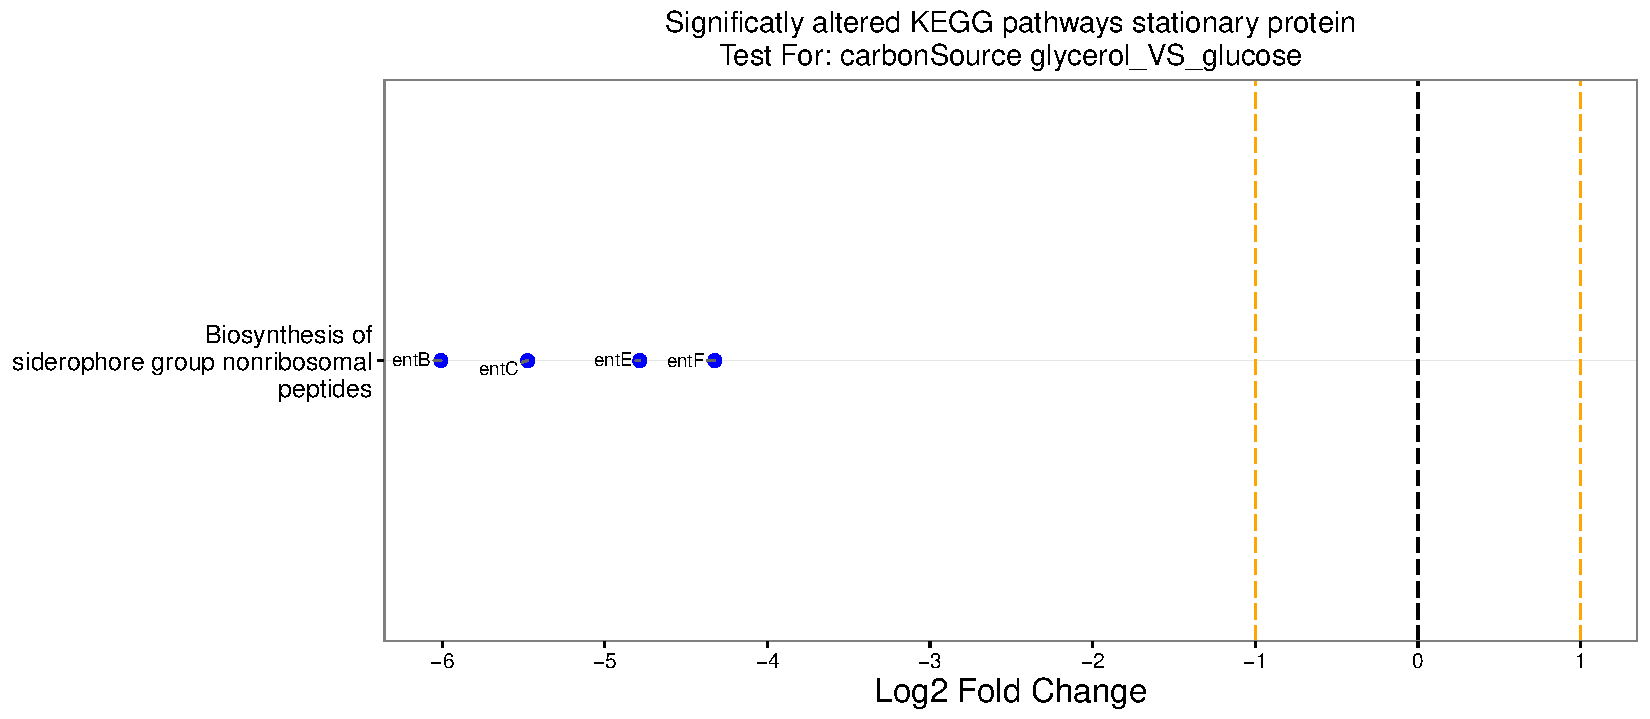
\includegraphics[width=1.0\textwidth]{../../d_figures/kegg_06.pdf}
	\caption[Significantly altered KEGG pathways for protein samples in stationary phase tested for glycerol against glucose]
	{\textbf{Significantly differentially expressed KEGG pathways and associated genes with glycerol as carbon source in stationary phase, as determined by protein abundances.} The top differentially expressed KEGG pathways are shown along the y axis, and the relative fold change of the corresponding genes is shown along the x axis. In figure we show up to 10 most significantly changed pathways and for each pathway, we show up to 15 of the most significantly changing genes.}
\end{figure}

\clearpage
\begin{figure}
	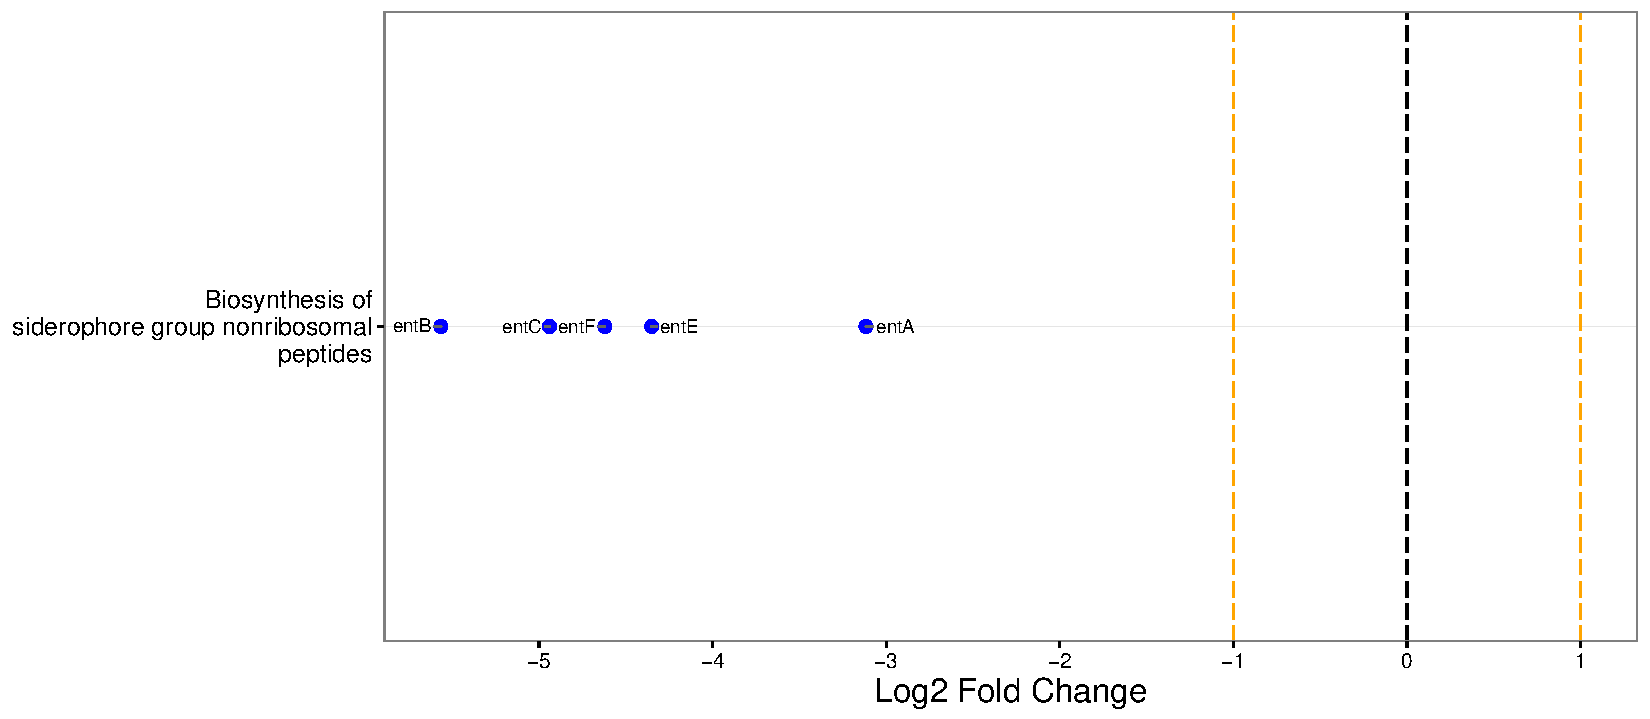
\includegraphics[width=1.0\textwidth]{../../d_figures/kegg_07.pdf}
	\caption[Significantly altered KEGG pathways for protein samples in stationary phase tested for gluconate against glucose]
	{\textbf{Significantly differentially expressed KEGG pathways and associated genes with gluconate as carbon source in stationary phase, as determined by protein abundances.} The top differentially expressed KEGG pathways are shown along the y axis, and the relative fold change of the corresponding genes is shown along the x axis. We show up to 10 most significantly changed pathways and for each pathway, we show up to 15 of the most significantly changing genes.}
\end{figure}

\clearpage
\begin{figure}
	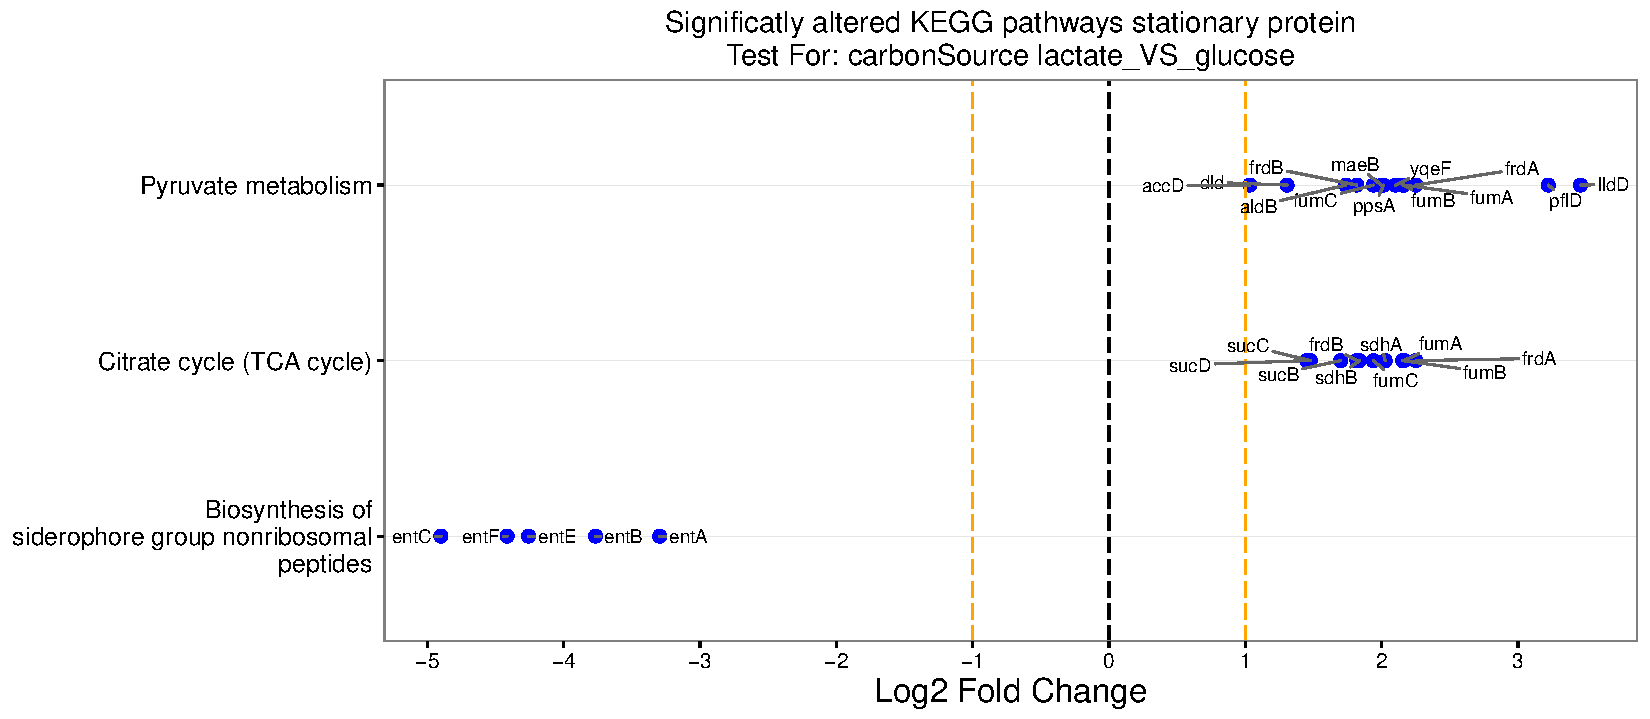
\includegraphics[width=1.0\textwidth]{../../d_figures/kegg_08.pdf}
	\caption[Significantly altered KEGG pathways for protein samples in stationary phase tested for lactate against glucose]
	{\textbf{Significantly differentially expressed KEGG pathways and associated genes with lactate as carbon source in stationary phase, as determined by protein abundances.} The top differentially expressed KEGG pathways are shown along the y axis, and the relative fold change of the corresponding genes is shown along the x axis. We show up to 10 most significantly changed pathways and for each pathway, we show up to 15 of the most significantly changing genes.}
\end{figure}

\clearpage
\begin{figure}
	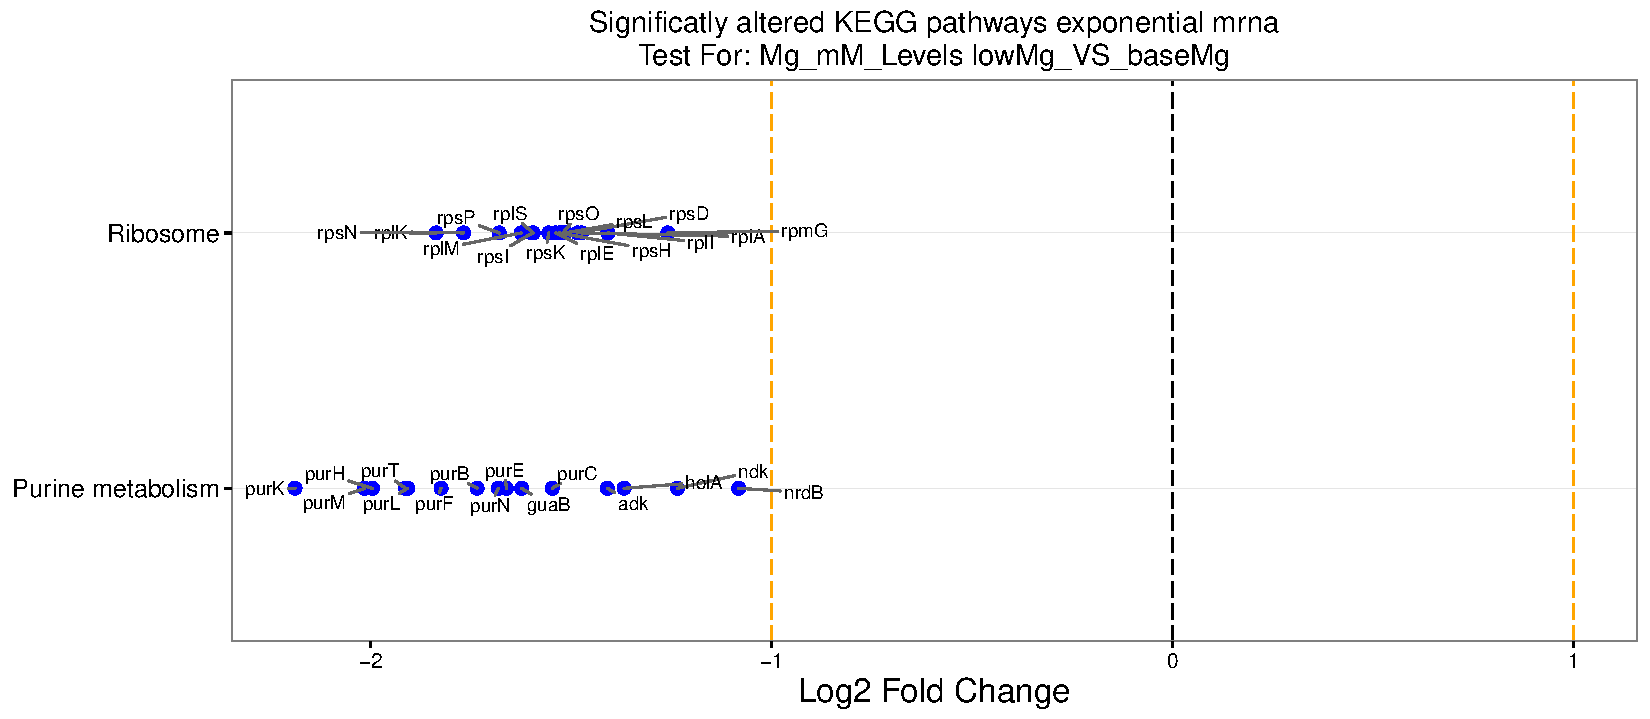
\includegraphics[width=1.0\textwidth]{../../d_figures/kegg_09.pdf}
	\caption[Significantly altered KEGG pathways for mRNA samples in exponential phase tested for low Mg\textsuperscript{+2} levels against base Mg\textsuperscript{+2}]
	{\textbf{Significantly differentially expressed KEGG pathways and associated genes with low Mg\textsuperscript{+2} levels in exponential phase, as determined by mRNA abundances.} The top differentially expressed KEGG pathways are shown along the y axis, and the relative fold change of the corresponding genes is shown along the x axis. We show up to 10 most significantly changed pathways and for each pathway, we show up to 15 of the most significantly changing genes.}
\end{figure}

\clearpage
\begin{figure}
	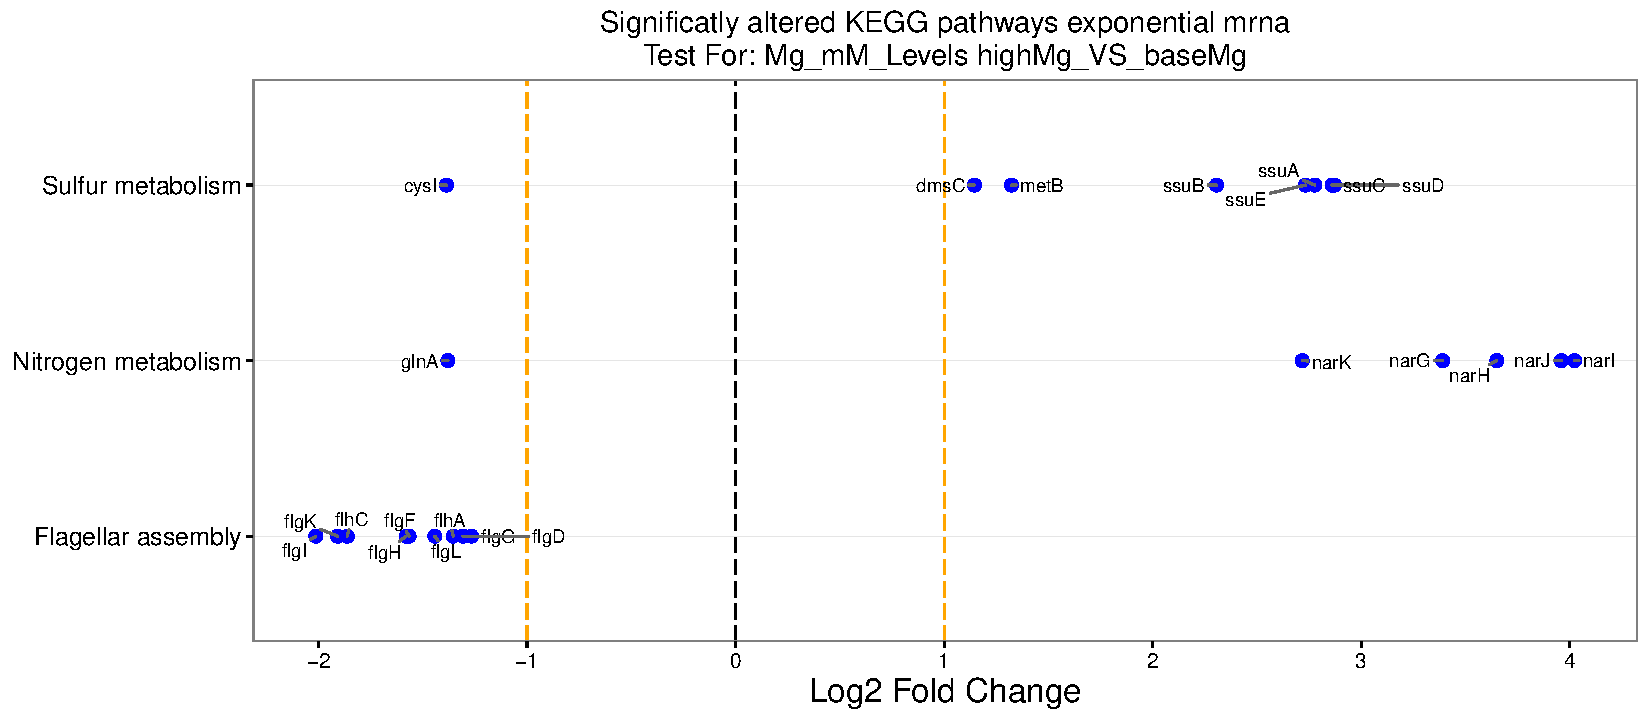
\includegraphics[width=1.0\textwidth]{../../d_figures/kegg_10.pdf}
	\caption[Significantly altered KEGG pathways for mRNA samples in exponential phase tested for high Mg\textsuperscript{+2} against base Mg\textsuperscript{+2}]
	{\textbf{Significantly differentially expressed KEGG pathways and associated genes with high Mg\textsuperscript{+2} levels in exponential phase, as determined by mRNA abundances.} The top differentially expressed KEGG pathways are shown along the y axis, and the relative fold change of the corresponding genes is shown along the x axis. We show up to 10 most significantly changed pathways and for each pathway, we show up to 15 of the most significantly changing genes.}
\end{figure}

\clearpage
\begin{figure}
	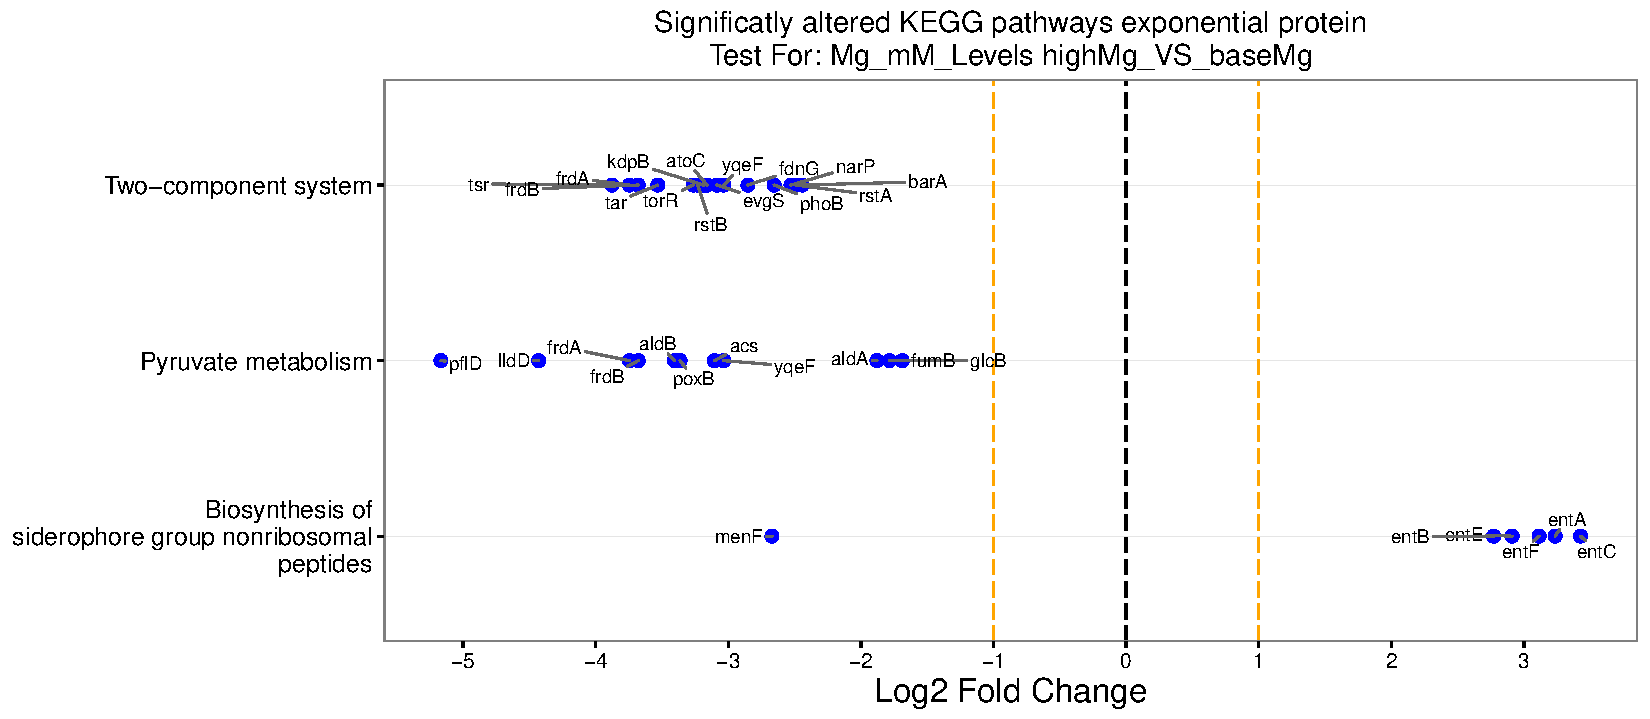
\includegraphics[width=1.0\textwidth]{../../d_figures/kegg_11.pdf}
	\caption[Significantly altered KEGG pathways for protein samples in exponential phase tested for high Mg\textsuperscript{+2} against base Mg\textsuperscript{+2}]
	{\textbf{Significantly differentially expressed KEGG pathways and associated genes with high Mg\textsuperscript{+2} levels in exponential phase, as determined by protein abundances.} The top differentially expressed KEGG pathways are shown along the y axis, and the relative fold change of the corresponding genes is shown along the x axis. We show up to 10 most significantly changed pathways and for each pathway, we show up to 15 of the most significantly changing genes.}
\end{figure}

\clearpage
\begin{figure}
	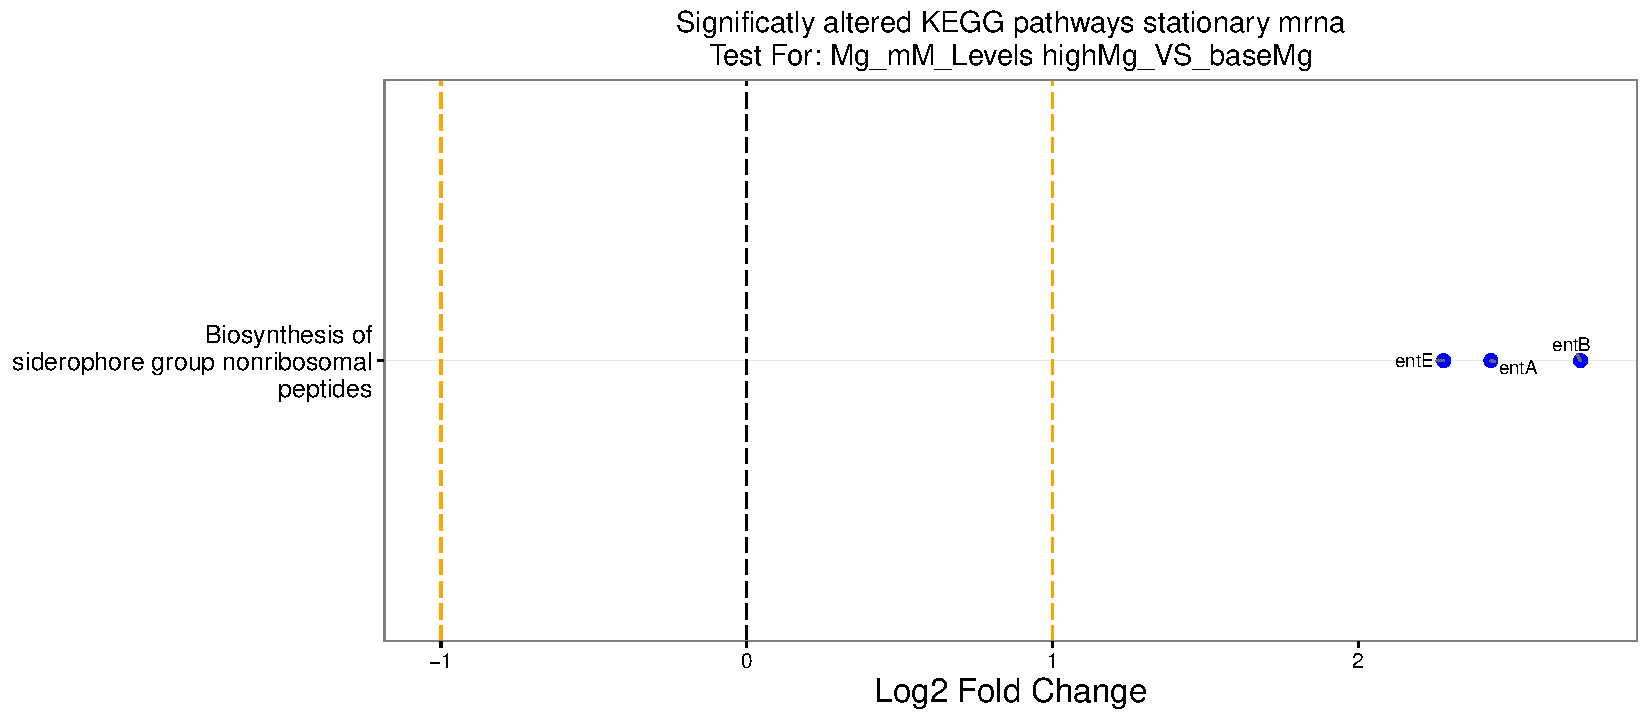
\includegraphics[width=1.0\textwidth]{../../d_figures/kegg_12.pdf}
	\caption[Significantly altered KEGG pathways for mRNA samples in stationary phase tested for high Mg\textsuperscript{+2} against base Mg\textsuperscript{+2}]
	{\textbf{Significantly differentially expressed KEGG pathways and associated genes with high Mg\textsuperscript{+2} levels in stationary phase, as determined by mRNA abundances.} The top differentially expressed KEGG pathways are shown along the y axis, and the relative fold change of the corresponding genes is shown along the x axis. We show up to 10 most significantly changed pathways and for each pathway, we show up to 15 of the most significantly changing genes.}
\end{figure}

\clearpage
\begin{figure}
	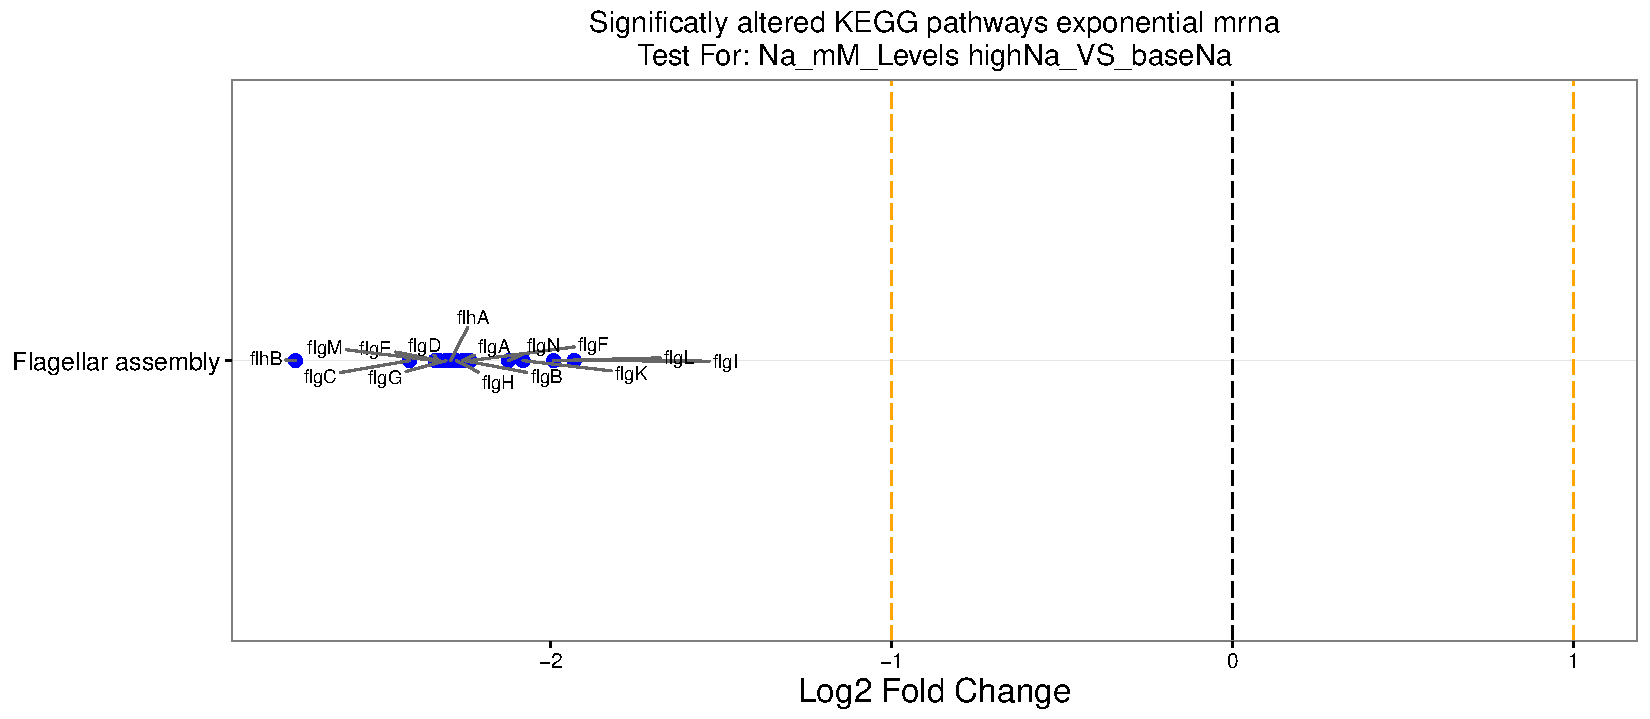
\includegraphics[width=1.0\textwidth]{../../d_figures/kegg_13.pdf}
	\caption[Significantly altered KEGG pathways for mRNA samples in exponential phase tested for high Na\textsuperscript{+1} against base Na\textsuperscript{+1}]
	{\textbf{Significantly differentially expressed KEGG pathways and associated genes with high Na\textsuperscript{+1} levels in exponential phase, as determined by mRNA abundances.} The top differentially expressed KEGG pathways are shown along the y axis, and the relative fold change of the corresponding genes is shown along the x axis. We show up to 10 most significantly changed pathways and for each pathway, we show up to 15 of the most significantly changing genes.}
\end{figure}

\clearpage
\begin{figure}
	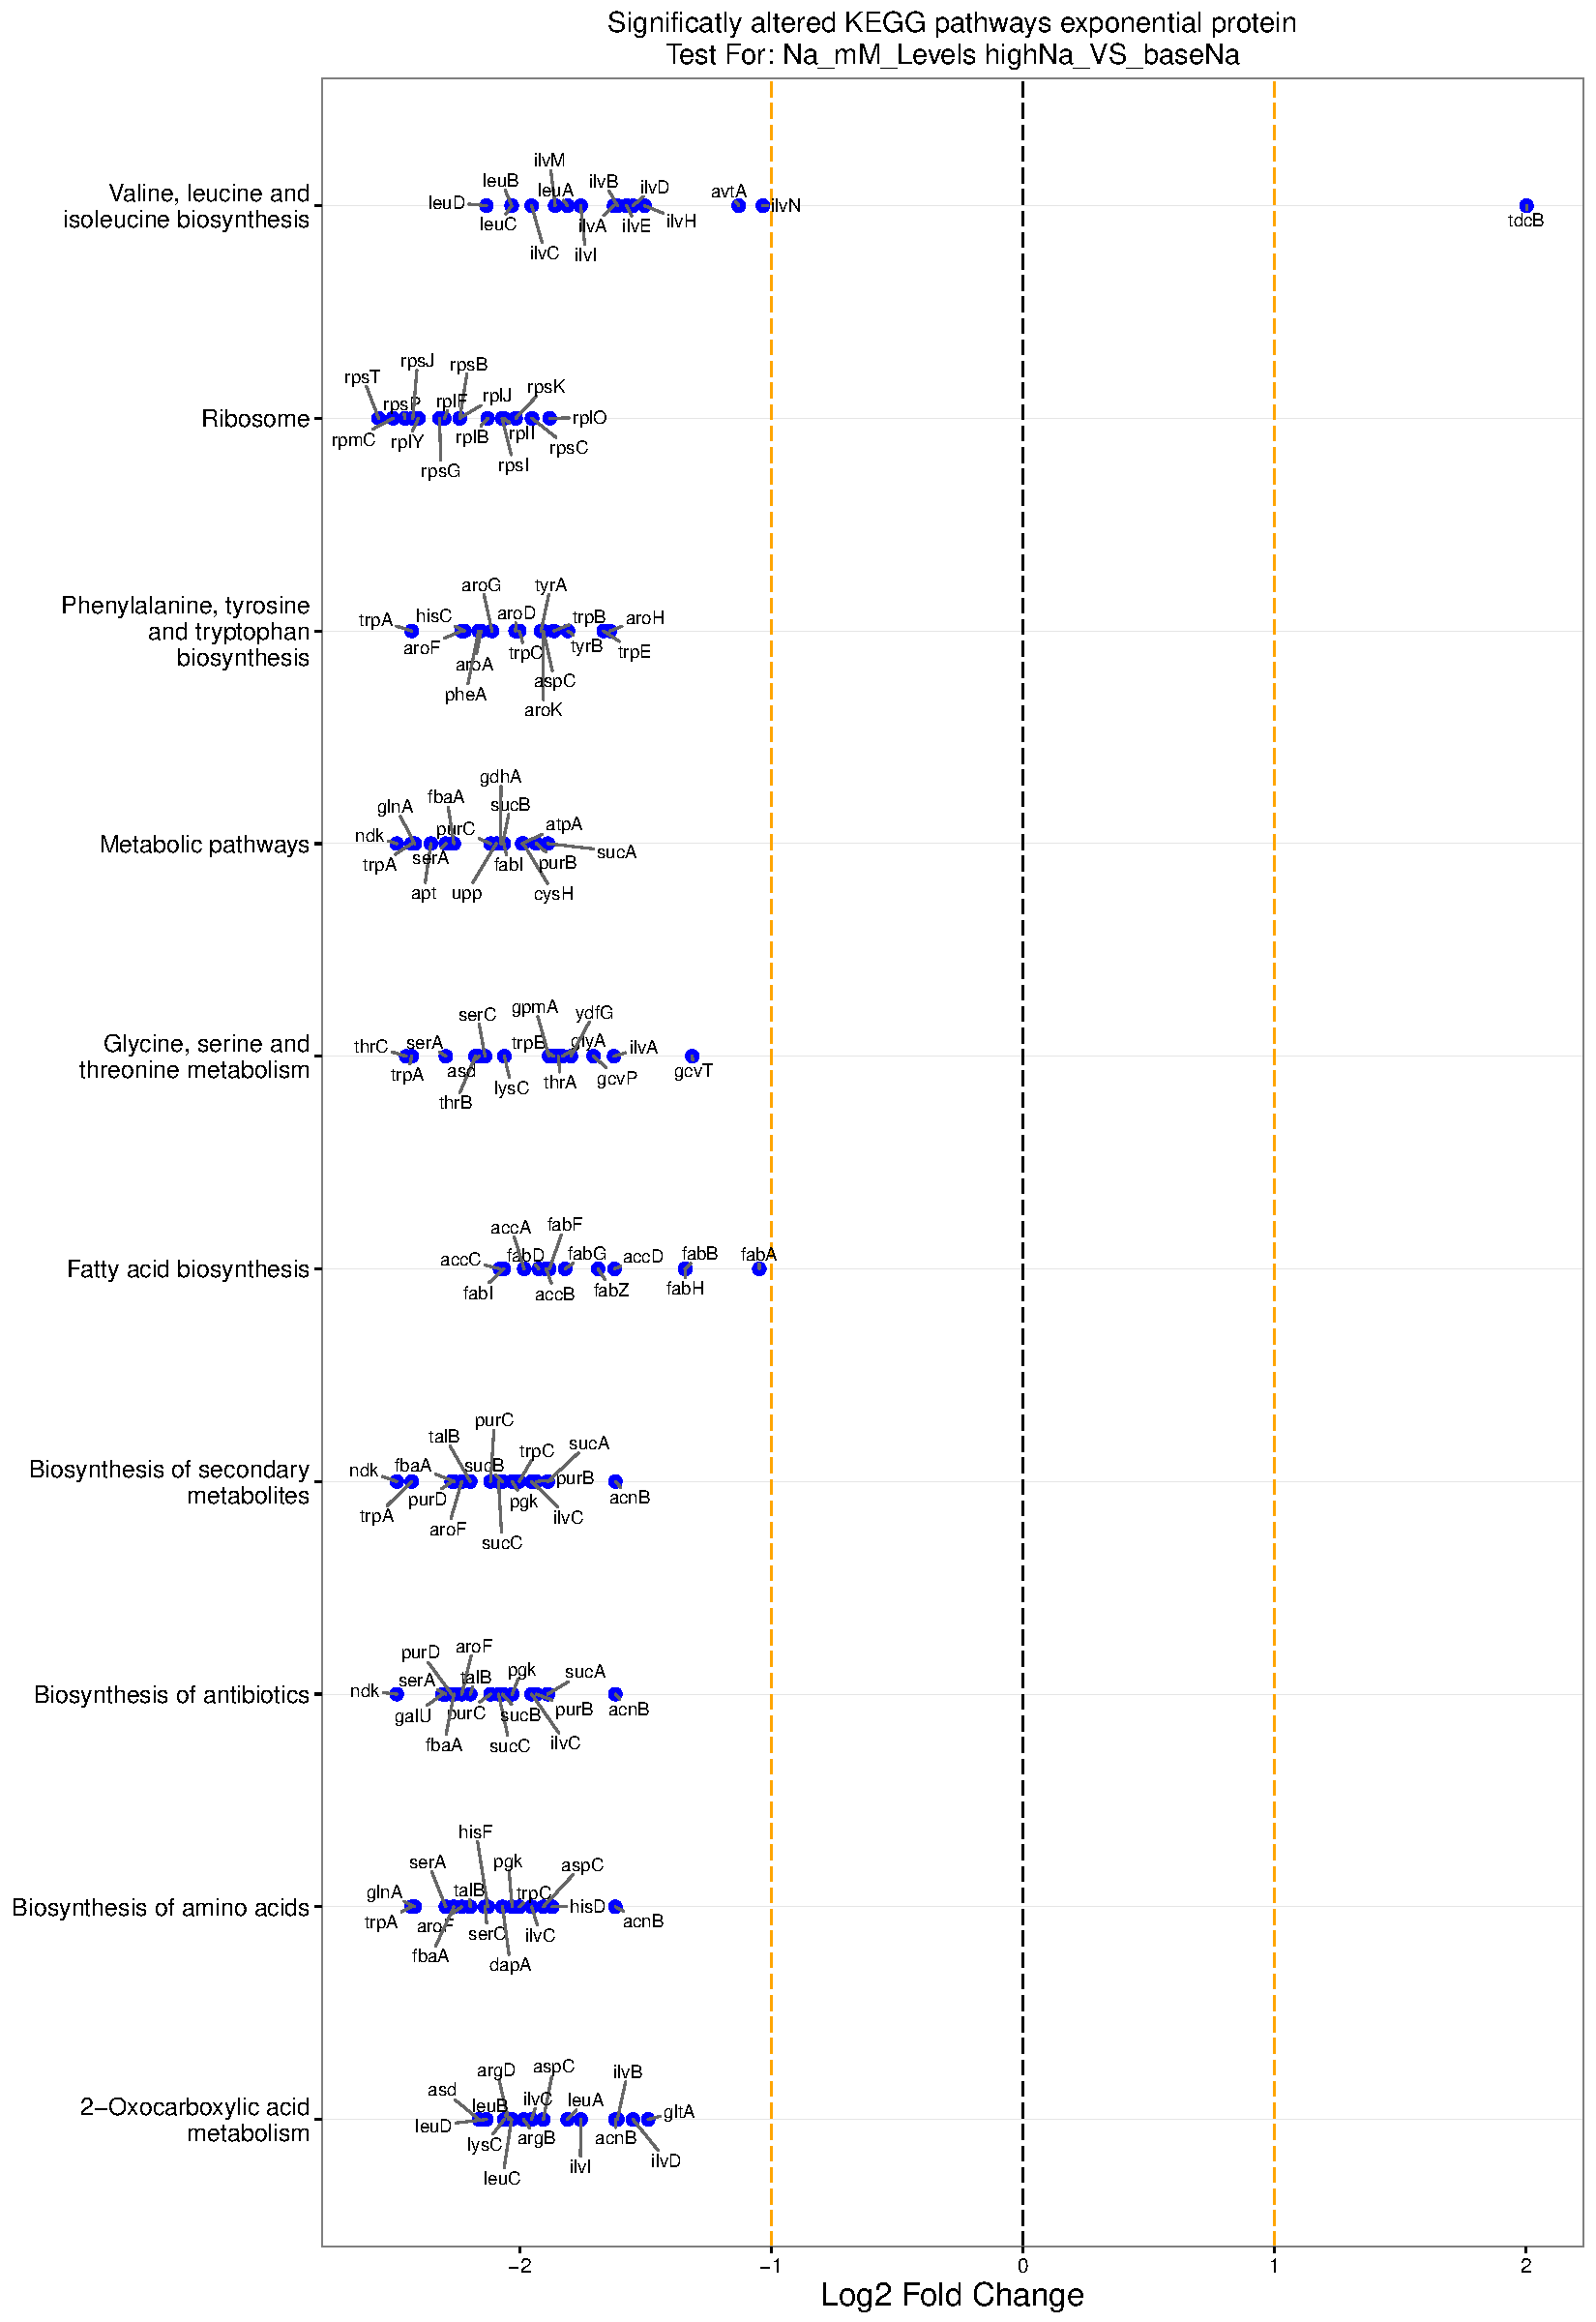
\includegraphics[width=1.0\textwidth]{../../d_figures/kegg_14.pdf}
	\caption[Significantly altered KEGG pathways for protein samples in exponential phase tested for high Na\textsuperscript{+1} against base Na\textsuperscript{+1}]
	{\textbf{Significantly differentially expressed KEGG pathways and associated genes with high Na\textsuperscript{+1} levels in exponential phase, as determined by protein abundances.} The top differentially expressed KEGG pathways are shown along the y axis, and the relative fold change of the corresponding genes is shown along the x axis. We show up to 10 most significantly changed pathways and for each pathway, we show up to 15 of the most significantly changing genes.}
\end{figure}

\clearpage
\begin{figure}
	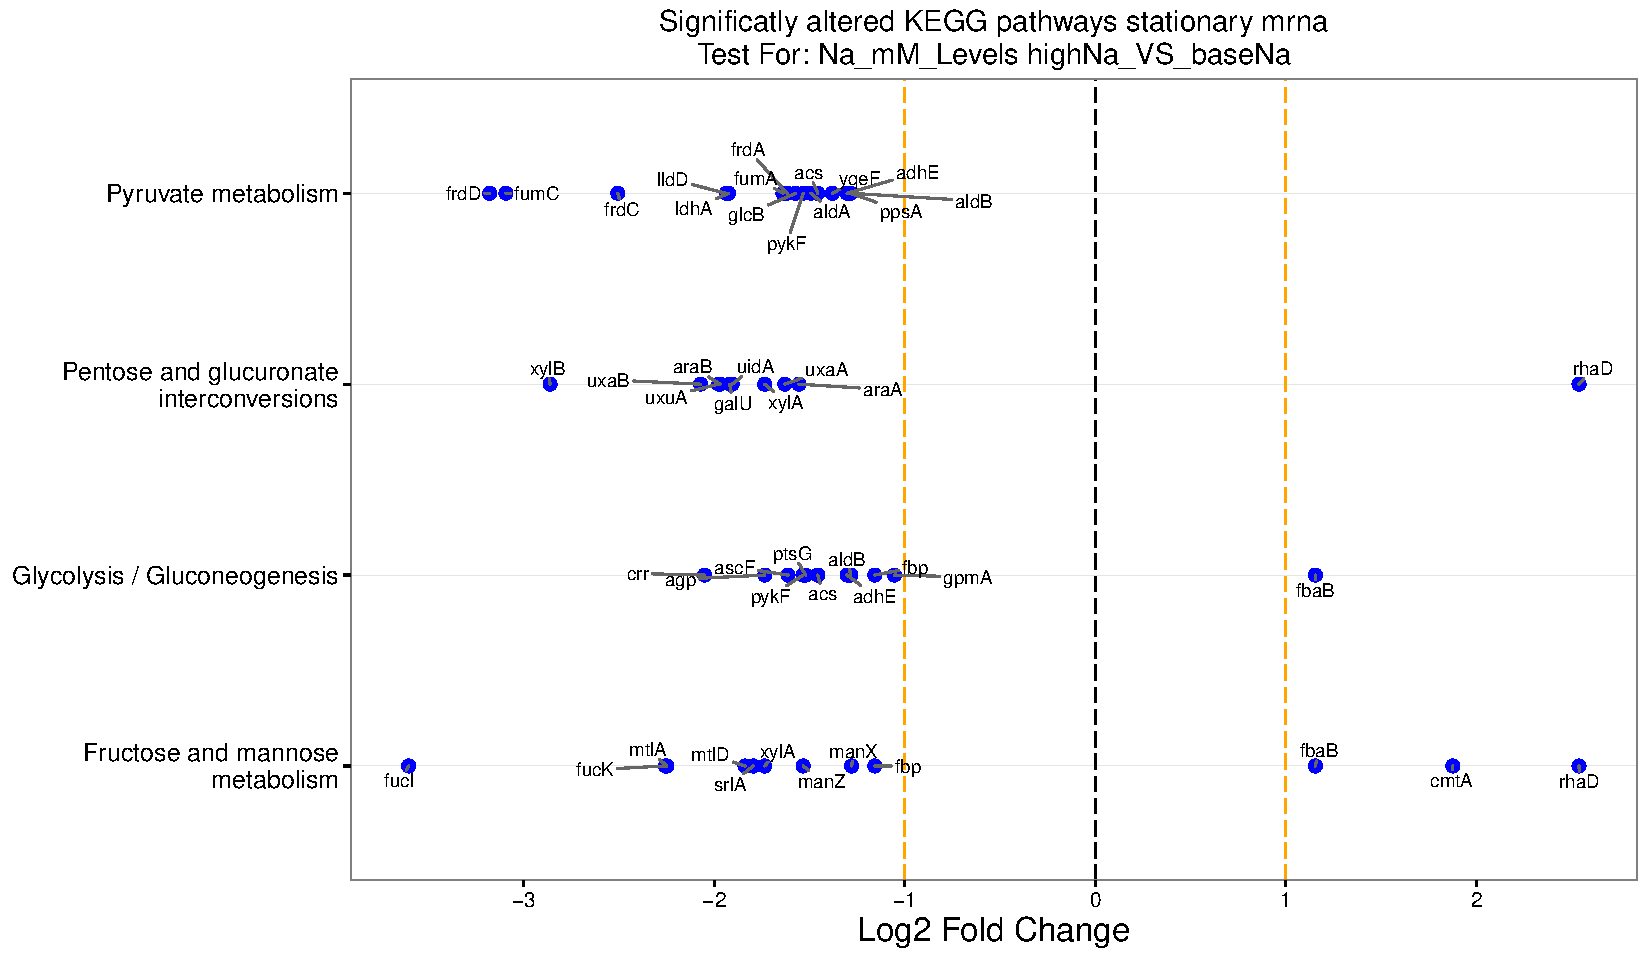
\includegraphics[width=1.0\textwidth]{../../d_figures/kegg_15.pdf}
	\caption[Significantly altered KEGG pathways for mRNA samples in stationary phase tested for high Na\textsuperscript{+1} against base Na\textsuperscript{+1}]
	{\textbf{Significantly differentially expressed KEGG pathways and associated genes with high Na\textsuperscript{+1} levels in stationary phase, as determined by mRNA abundances.} The top differentially expressed KEGG pathways are shown along the y axis, and the relative fold change of the corresponding genes is shown along the x axis. We show up to 10 most significantly changed pathways and for each pathway, we show up to 15 of the most significantly changing genes.}
\end{figure}

\clearpage
\begin{figure}
	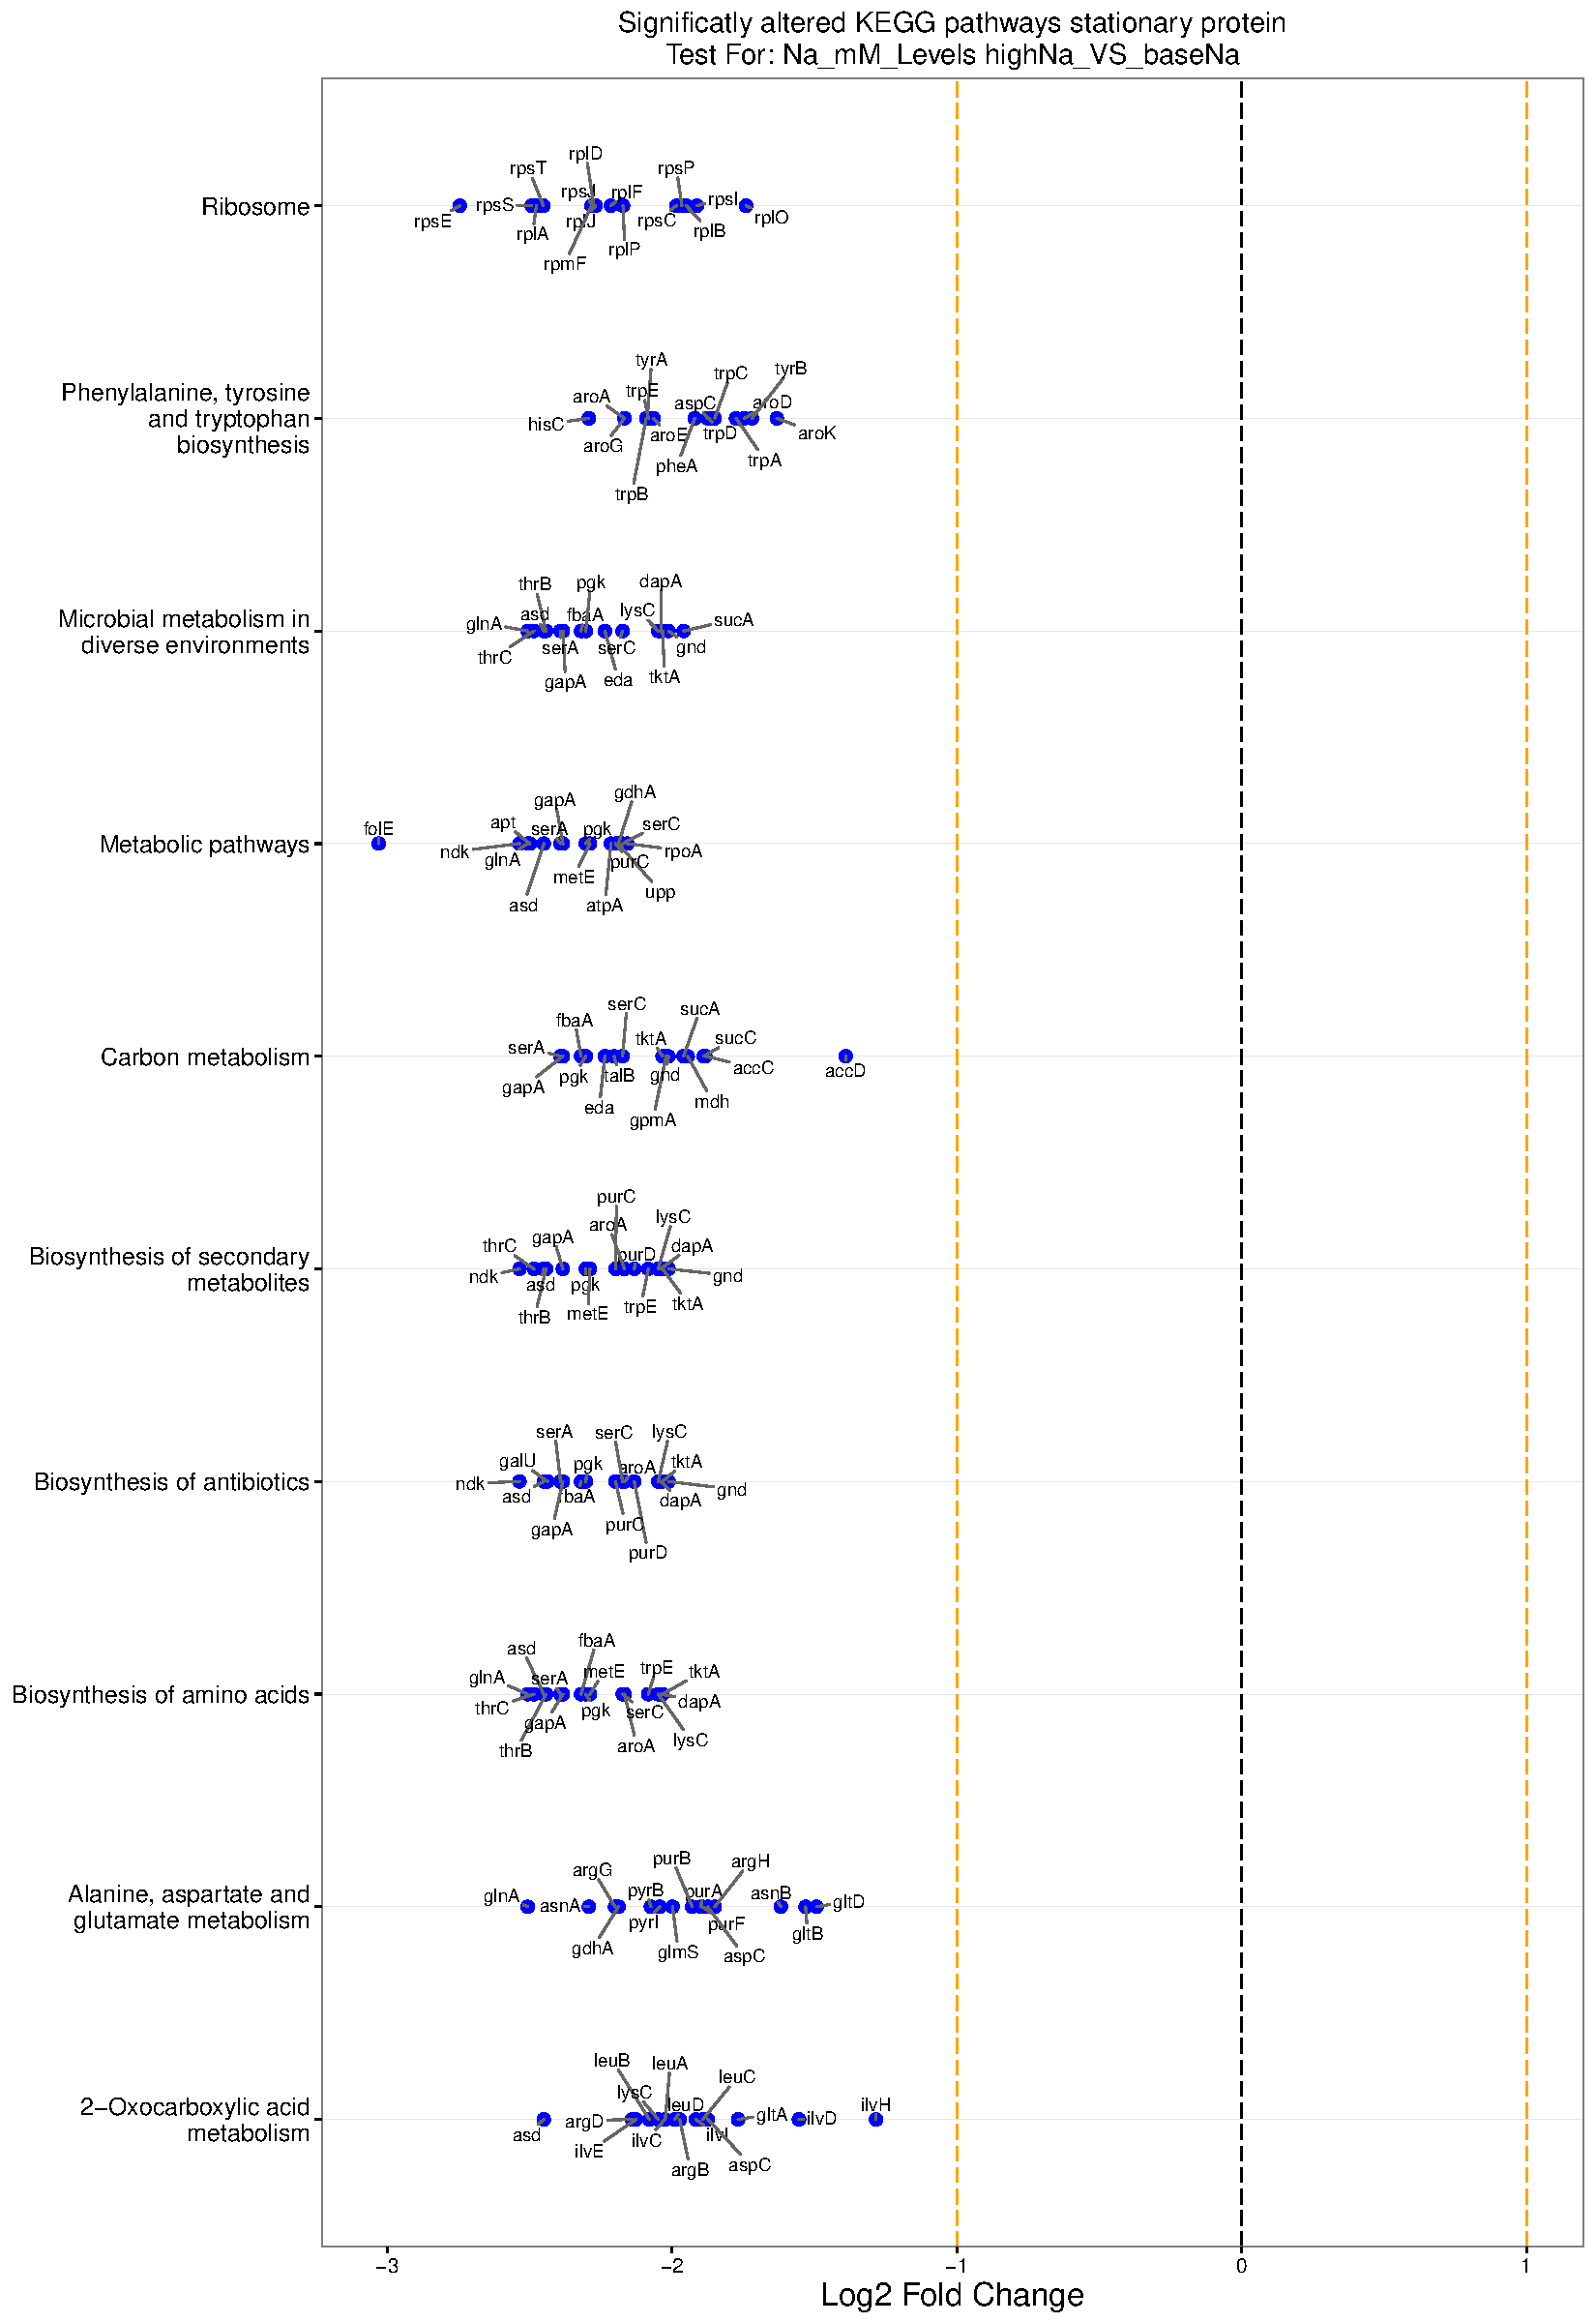
\includegraphics[width=1.0\textwidth]{../../d_figures/kegg_16.pdf}
	\caption[Significantly altered KEGG pathways for protein samples in stationary phase tested for high Na\textsuperscript{+1} against base Na\textsuperscript{+1}]
	{\textbf{Significantly differentially expressed KEGG pathways and associated genes with high Na\textsuperscript{+1} levels in stationary phase, as determined by protein abundances.} The top differentially expressed KEGG pathways are shown along the y axis, and the relative fold change of the corresponding genes is shown along the x axis. We show up to 10 most significantly changed pathways and for each pathway, we show up to 15 of the most significantly changing genes.}
\end{figure}
\clearpage

\section*{Supplementary Figures related with GO Annotations associated with Molecular Function}

\begin{figure}[!htb]
	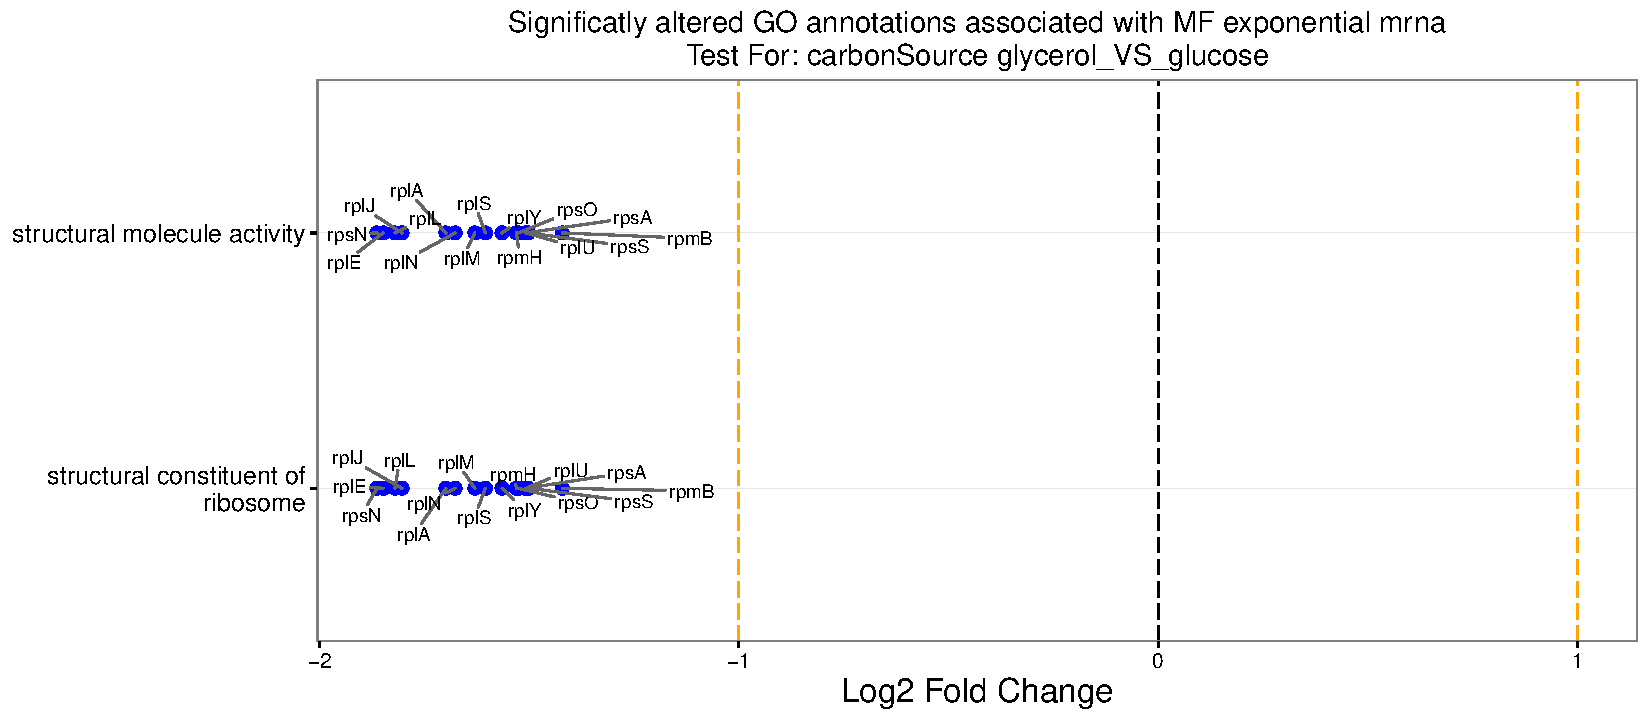
\includegraphics[width=1.0\textwidth]{../../d_figures/mf_n_01.pdf}
	\caption[Significantly altered GO annotations associated with molecular functions for mRNA samples in exponential phase tested for glycerol against glucose]
	{\textbf{Significantly differentially expressed GO annotations related with molecular functions and associated genes with glycerol as carbon source in exponential phase, as determined by mRNA abundances.} The top differentially expressed KEGG pathways are shown along the y axis, and the relative fold change of the corresponding genes is shown along the x axis. We show up to 10 most significantly changed pathways and for each pathway, we show up to 15 of the most significantly changing genes.}
\end{figure}

\clearpage
\begin{figure}
	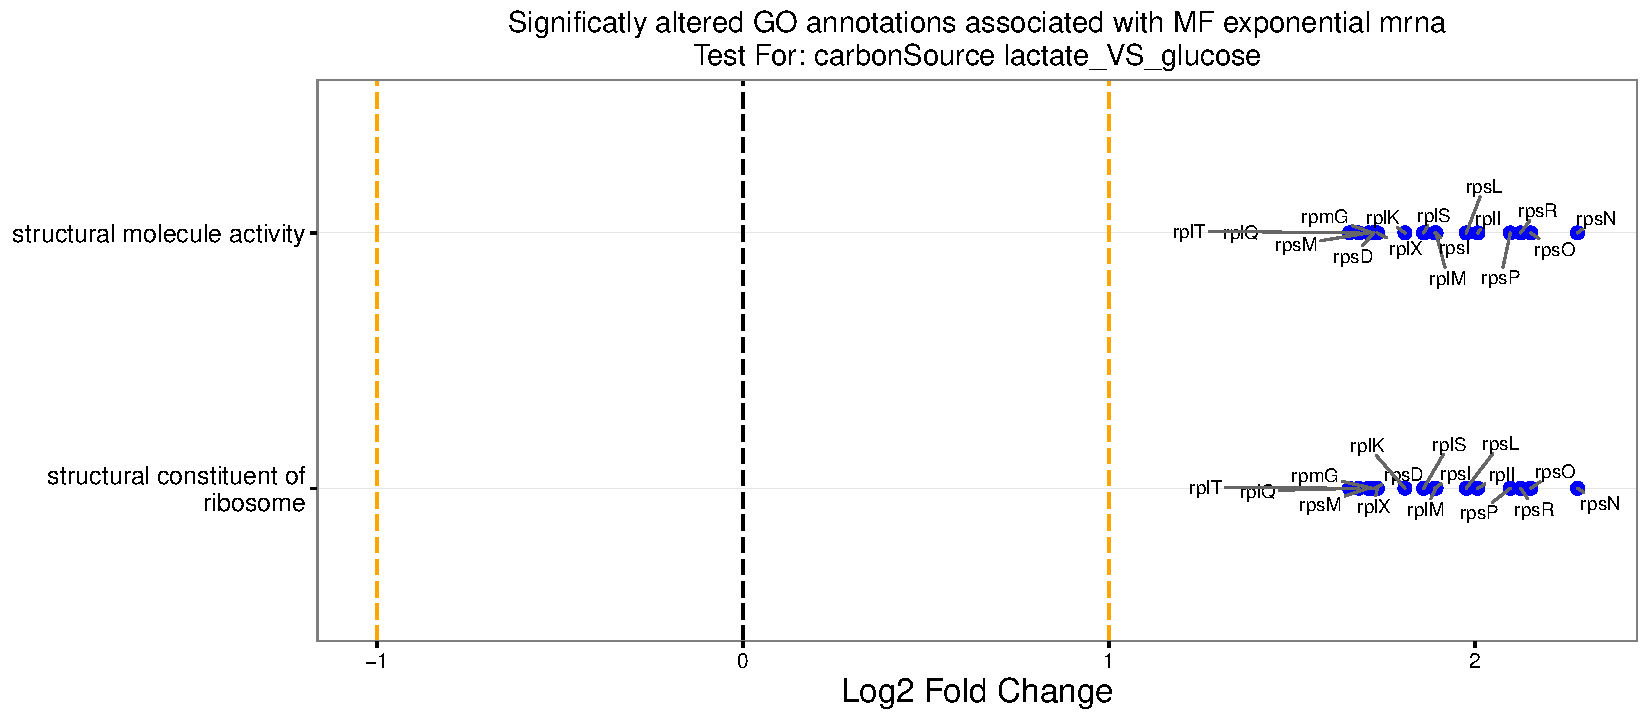
\includegraphics[width=1.0\textwidth]{../../d_figures/mf_n_02.pdf}
	\caption[Significantly altered GO annotations associated with molecular functions for mRNA samples in exponential phase tested for lactate against glucose]
	{\textbf{Significantly differentially expressed GO annotations related with molecular functions and associated genes with lactate as carbon source in exponential phase, as determined by mRNA abundances.} The top differentially expressed KEGG pathways are shown along the y axis, and the relative fold change of the corresponding genes is shown along the x axis. We show up to 10 most significantly changed pathways and for each pathway, we show up to 15 of the most significantly changing genes.}
\end{figure}

\clearpage
\begin{figure}
	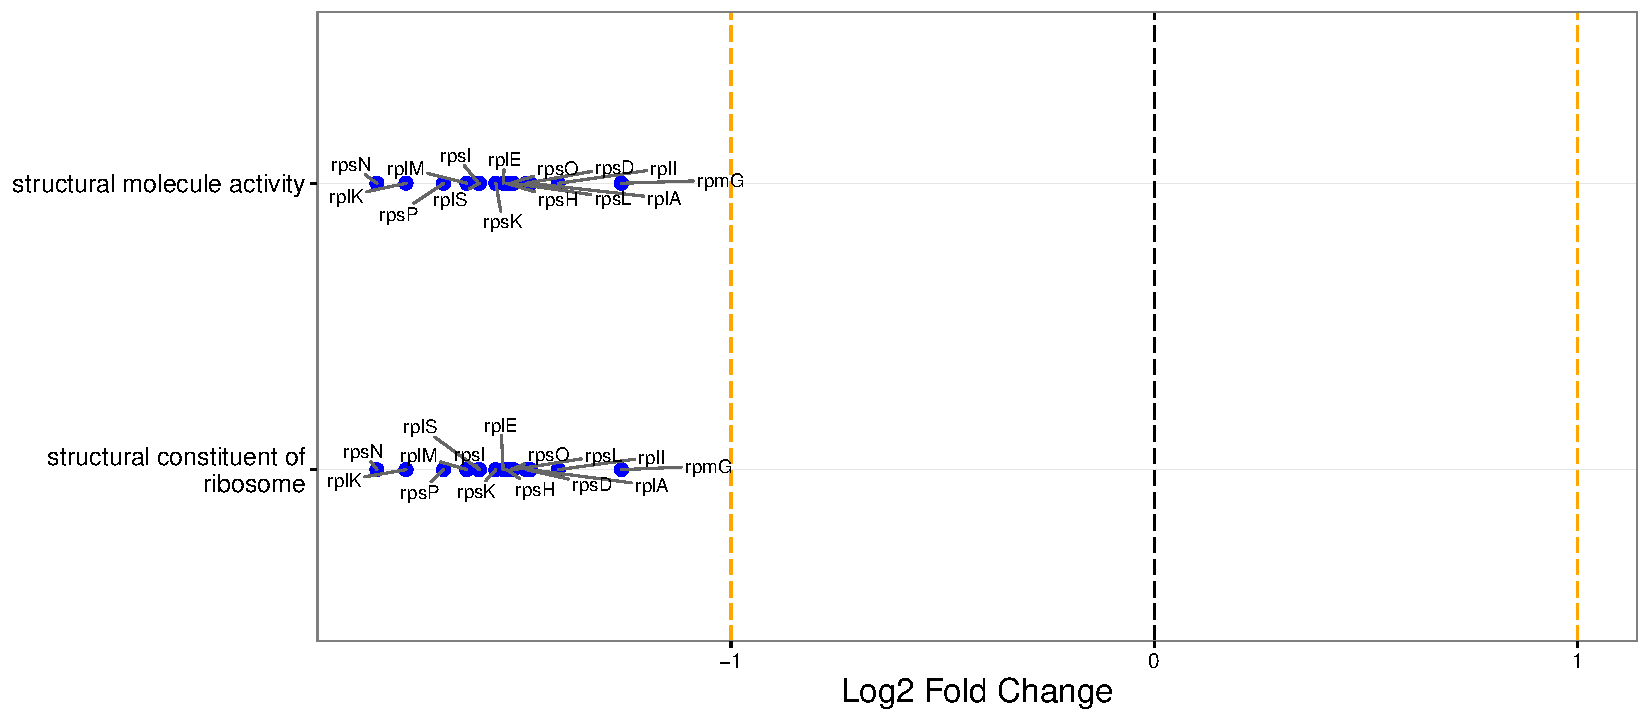
\includegraphics[width=1.0\textwidth]{../../d_figures/mf_n_03.pdf}
	\caption[Significantly altered GO annotations associated with molecular functions for mRNA samples in exponential phase tested for low Mg\textsuperscript{+2} against base Mg\textsuperscript{+2}]
	{\textbf{Significantly differentially expressed GO annotations related with molecular functions and associated genes with low Mg\textsuperscript{+2} levels in exponential phase, as determined by mRNA abundances.} The top differentially expressed KEGG pathways are shown along the y axis, and the relative fold change of the corresponding genes is shown along the x axis. We show up to 10 most significantly changed pathways and for each pathway, we show up to 15 of the most significantly changing genes.}
\end{figure}

\clearpage
\begin{figure}
	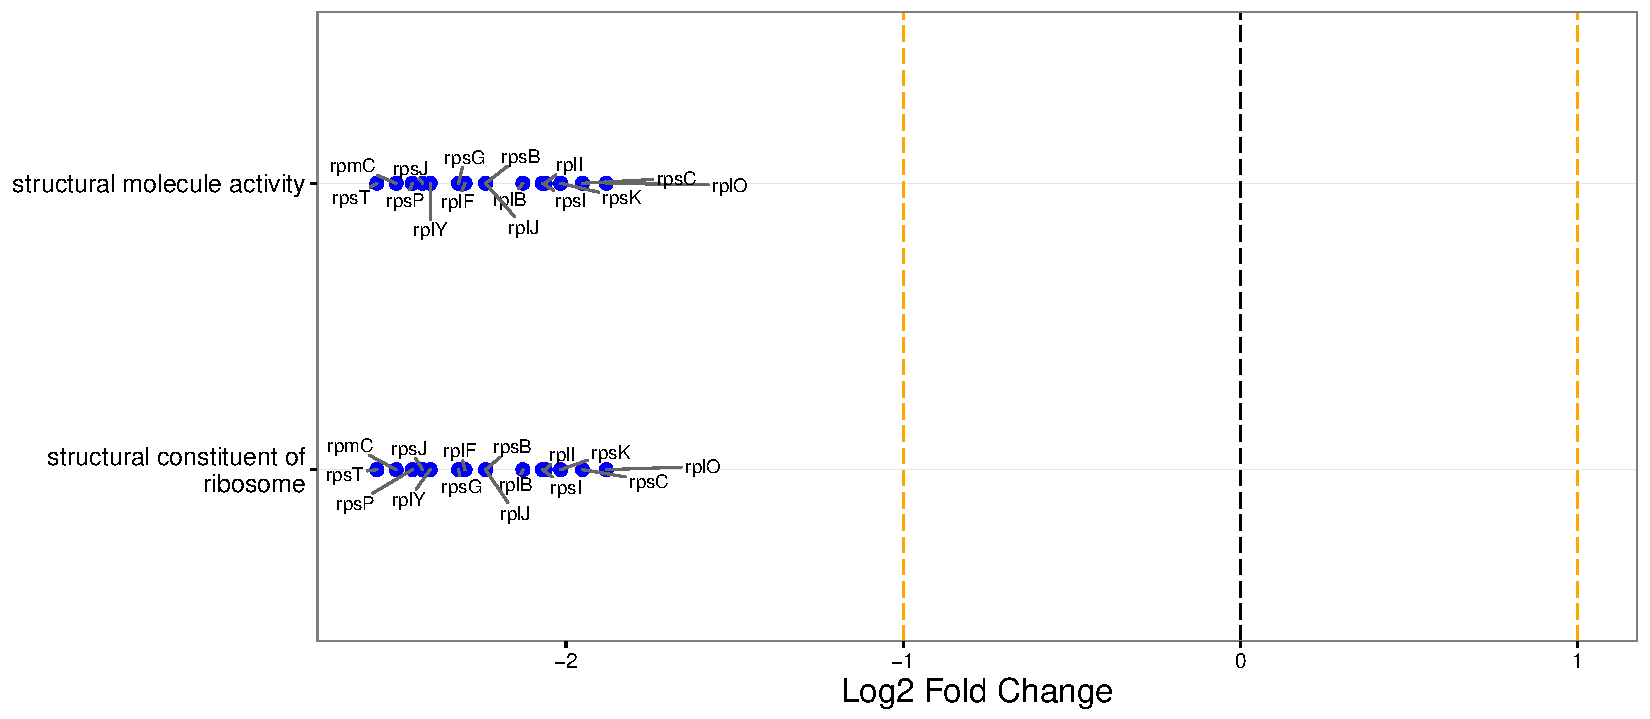
\includegraphics[width=1.0\textwidth]{../../d_figures/mf_n_04.pdf}
	\caption[Significantly altered GO annotations associated with molecular functions for protein samples in exponential phase tested for high Na\textsuperscript{+1} against base Na\textsuperscript{+1}]
	{\textbf{Significantly differentially expressed GO annotations related with molecular functions and associated genes with high Na\textsuperscript{+1} levels in exponential phase, as determined by protein abundances.} The top differentially expressed KEGG pathways are shown along the y axis, and the relative fold change of the corresponding genes is shown along the x axis. We show up to 10 most significantly changed pathways and for each pathway, we show up to 15 of the most significantly changing genes.}
\end{figure}

\clearpage
\begin{figure}
	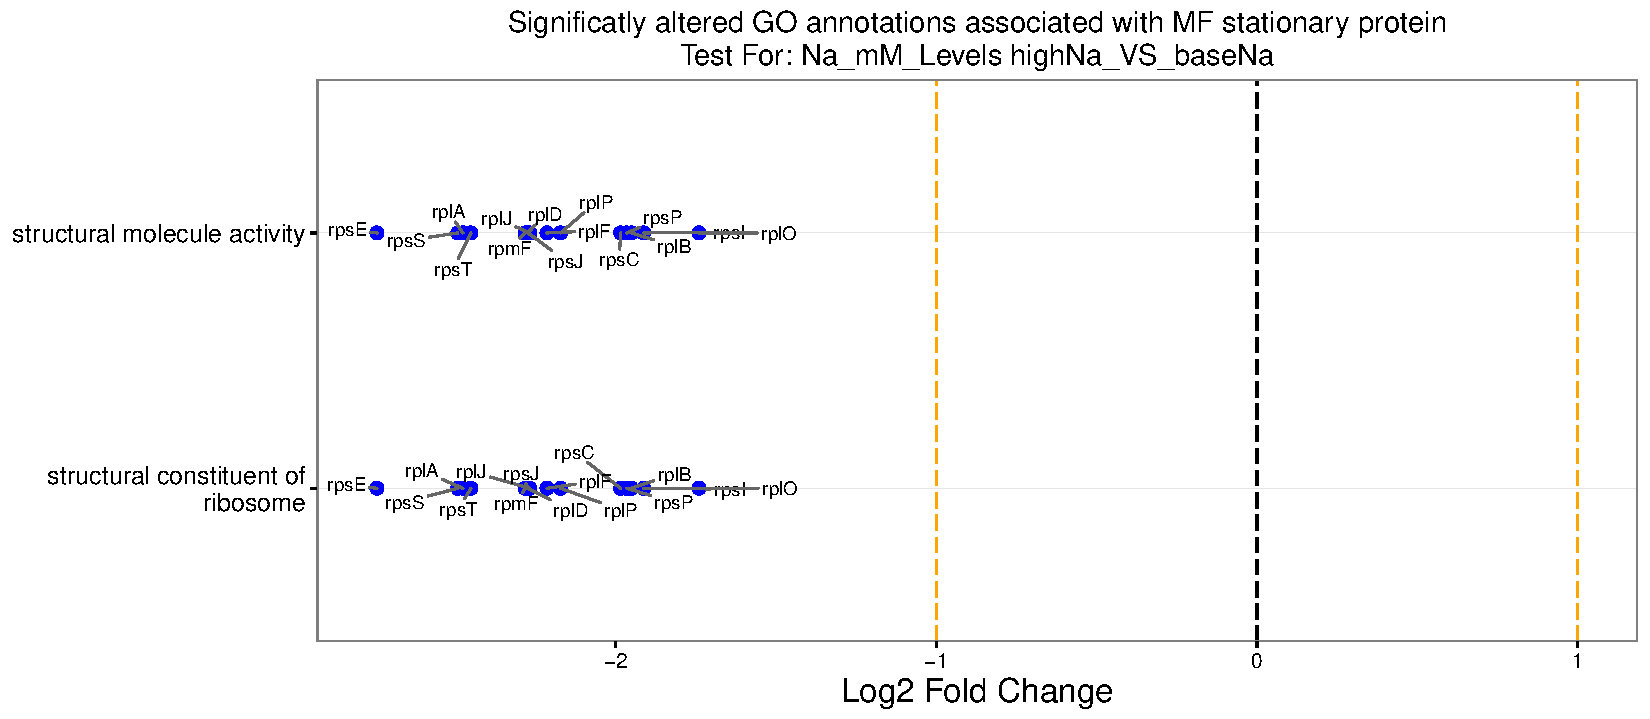
\includegraphics[width=1.0\textwidth]{../../d_figures/mf_n_05.pdf}
	\caption[Significantly altered GO annotations associated with molecular functions for protein samples in stationary phase tested for high Na\textsuperscript{+1} against base Na\textsuperscript{+1}]
	{\textbf{Significantly differentially expressed GO annotations related with molecular functions and associated genes with high Na\textsuperscript{+1} levels in stationary phase, as determined by protein abundances.} The top differentially expressed KEGG pathways are shown along the y axis, and the relative fold change of the corresponding genes is shown along the x axis. We show up to 10 most significantly changed pathways and for each pathway, we show up to 15 of the most significantly changing genes.}
\end{figure}



\clearpage
\section{Introduction}

Your introduction goes here! Some examples of commonly used commands and features are listed below, to help you get started. If you have a question, please use the help menu (``?'') on the top bar to search for help or ask us a question. 

\section{Some examples to get started}

\subsection{How to include Figures}

First you have to upload the image file from your computer using the upload link the project menu. Then use the includegraphics command to include it in your document. Use the figure environment and the caption command to add a number and a caption to your figure. See the code for Figure \ref{fig:frog} in this section for an example.

\begin{figure}
\centering
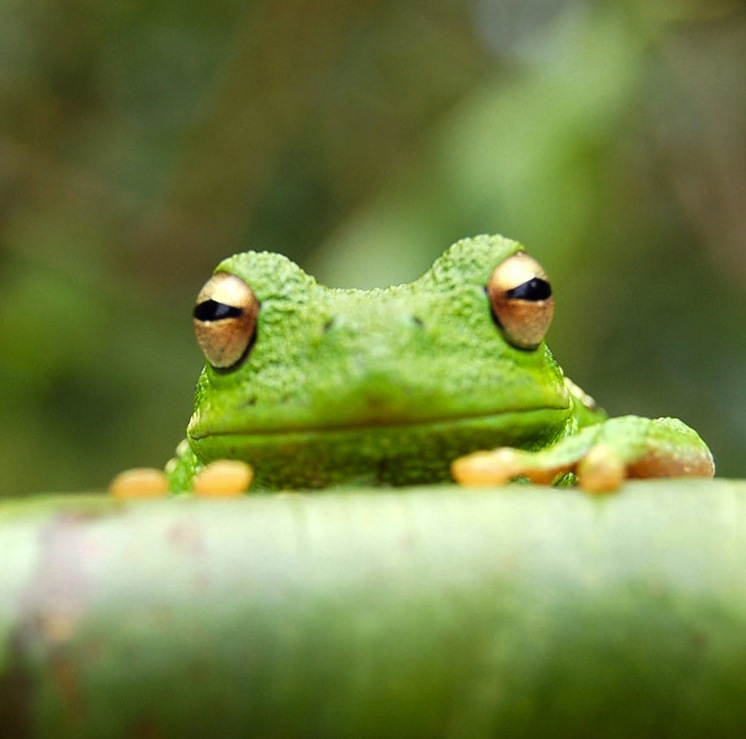
\includegraphics[width=0.3\textwidth]{frog.jpg}
\caption{\label{fig:frog}This frog was uploaded via the project menu.}
\end{figure}

\subsection{How to add Comments}

Comments can be added to your project by clicking on the comment icon in the toolbar above. % * <john.hammersley@gmail.com> 2016-07-03T09:54:16.211Z:
%
% Here's an example comment!
%
To reply to a comment, simply click the reply button in the lower right corner of the comment, and you can close them when you're done.

Comments can also be added to the margins of the compiled PDF using the todo command, \todo{Here's a comment in the margin!} as shown in the example on the right. You can also add inline comments:

\todo[inline, color=green!40]{This is an inline comment.}

\subsection{How to add Tables}

Use the table and tabular commands for basic tables --- see Table~\ref{tab:widgets}, for example. 

\begin{table}
\centering
\begin{tabular}{l|r}
Item & Quantity \\\hline
Widgets & 42 \\
Gadgets & 13
\end{tabular}
\caption{\label{tab:widgets}An example table.}
\end{table}

\subsection{How to write Mathematics}

\LaTeX{} is great at typesetting mathematics. Let $X_1, X_2, \ldots, X_n$ be a sequence of independent and identically distributed random variables with $\text{E}[X_i] = \mu$ and $\text{Var}[X_i] = \sigma^2 < \infty$, and let
\[S_n = \frac{X_1 + X_2 + \cdots + X_n}{n}
      = \frac{1}{n}\sum_{i}^{n} X_i\]
denote their mean. Then as $n$ approaches infinity, the random variables $\sqrt{n}(S_n - \mu)$ converge in distribution to a normal $\mathcal{N}(0, \sigma^2)$.


\subsection{How to create Sections and Subsections}

Use section and subsections to organize your document. Simply use the section and subsection buttons in the toolbar to create them, and we'll handle all the formatting and numbering automatically.

\subsection{How to add Lists}

You can make lists with automatic numbering \dots

\begin{enumerate}
\item Like this,
\item and like this.
\end{enumerate}
\dots or bullet points \dots
\begin{itemize}
\item Like this,
\item and like this.
\end{itemize}

We hope you find Overleaf useful, and please let us know if you have any feedback using the help menu above.

\end{document}